% This template was written by John Davies <john.davies@glasgow.ac.uk> 2017-02-06
% It matches the university specification at the time of writing
%   for the widths of the page margins and one-and-a-half line spacing
% You may want to include more packages, particularly for heavy mathematics
% Please let me know if you find any errors or wish to suggest improvements

\documentclass[12pt,titlepage,oneside]{book}
\usepackage[T1]{fontenc} % modern encoding
% Comment out the next three lines of LaTeX if you wish to use Computer Modern fonts
%   (this is the default for LaTeX)
% Make sure that your TeX installation can produce good pdf with these fonts.
% The following three lines are a good alternative if you don't use much mathematics
\usepackage{mathptmx}  % uses Times for text and mathematics
\usepackage[scaled]{helvet} %  helvetica for sanserif, scaled 95% by default
%\usepackage{courier}  % courier for typewriter font, pretty ugly but available
% otherwise the stix package offers more options and symbols
\usepackage{stix}  % uses Times for text and a range of fonts for mathematics
% End of choices for fonts
\usepackage{graphicx}  % standard package for importing graphics files
%\usepackage{cite}  % improves format of numerical citations, such as [1-3]
\usepackage[top=1.8cm, bottom=1.8cm,left=4.0cm,right=1.5cm]{geometry}
% These margins are the university guidelines
\usepackage[onehalfspacing]{setspace}  % gives one-and-a-half line spacing
% doublespacing is another option and can be changed in the text

%% --- user packages ---

\usepackage{csquotes}
\usepackage{bm}
\usepackage{amsmath}
\usepackage{subcaption}
\usepackage{booktabs}
\usepackage{grffile}
\usepackage{overpic}

\usepackage[backend=biber]{biblatex}
\addbibresource{thesis.bib}

\usepackage{lineno,hyperref}
%\modulolinenumbers[5]

% Url style
\hypersetup{
    colorlinks=true,
    linkcolor=blue,
    filecolor=magenta,      
    urlcolor=cyan,
}
 
\urlstyle{same}

% For editing
\usepackage{color}
\newcommand{\rr}[1]{\textcolor{red}{#1}}
\newcommand{\bb}[1]{\textcolor{blue}{#1}}
\newcommand{\rs}[1]{\textcolor{blue}{#1}}
%\newcommand{\rr}[1]{#1}
%\newcommand{\bb}[1]{#1}
%\newcommand{\rs}[1]{#1}

%% --- user commands ---

\newcommand{\ten}[1]{{\bm #1}}
\renewcommand{\vec}[1]{{\bm #1}}

%% --- end user commands ---

\begin{document}
\begin{titlepage}
\centering
\vspace*{3cm}  % Need the * or the space is swallowed at the top of the page
\bfseries\Large
Anisotropic Viscosity and Astrophysical Applications\\
\vspace{3cm}
\normalfont\large
James Quinn\\
\vspace{2cm}
Submitted in fulfilment of the requirements for the\\
Degree of Doctor of Philosophy\\
\vspace{2cm}
School of Mathematics and Statistics\\
College of Science and Engineering\\
University of Glasgow\\
\vspace{1cm}
\includegraphics[scale=0.125]{GlaLogo.pdf}
\\
\vspace{1cm}
% Insert month and year of date deposited with library for final version
July 2020
\end{titlepage}
\frontmatter  % Turn off chapter numbering, use roman page numbers

Column width is \the\columnwidth

\chapter{Abstract}

Current understanding of the solar corona is plagued by what is known as the coronal heating problem--it is unknown how the solar atmosphere maintains a temperature of several orders of magnitude greater than that of the solar surface. Viscosity provides one mechanism by which  heat is generated, through the dissipation of kinetic energy. Although Newtonian viscosity is a common feature of many coronal simulations, the proper form of viscosity in a highly magnetised plasma is anisotropic and strongly coupled to the local magnetic field. This thesis investigates the differences between Newtonian and a novel model of anisotropic viscosity, the switching model, when applied to a simulations of the kink instability in a coronal loop, a slowly stressed magnetic null point, and the Kelvin-Helmholtz instability in the fan plane of a null point. Generally it's found that Newtonian viscosity overestimates the viscous heating by up to two orders of magnitude and can suppress the growth of instabilities and current sheets, leading to notably diminished Ohmic heating and reconnection rates.

\tableofcontents
\listoftables
\listoffigures
\chapter{Acknowledgements}

Thank you to everyone who has supported me during throughout my PhD. 

\vspace{5mm}

This research would not have been possible without the support and guidance from my supervisors, David MacTaggart, and Radostin Simitev. David, thank you for your patience and continual feedback. You've given an immense amount of time and energy to guiding my research, you've provided focus and insight and you've nurtured in me a thoroughness I did not previously possess. Rado, you've been a mentor, a stoic mediator and an inspiration. If I end up with a career half as illustrious as yours I will be happy.

Thank you also to the staff of the school of Maths \& Stats, in particular Dave for sorting out many a digital niggle; Jean, Margaret, Pauline, and Sharon for the care they take in dealing with every minutiae of admin; and Steve and Rob for convincing me to stick through the tough periods.

I would also like to thank the EPSRC for supporting me financially through my PhD, and the group behind ARCHIE-WeSt at the University of Strathclyde for their work in supporting the computational needs of Glasgow's academia.

\vspace{5mm}

I would be much closer to mental ruin without the support of my parents, Maureen and Patrick, and my partner in crime, Annie. Mum and Dad, thank you for encouraging me to choose my own path and pretending to know what I'm talking about when I warble on about the solar atmosphere. Annie, you make me food and make me laugh. Thank you for being who you are.

\vspace{5mm}

To my fellow PhD students in the School of Maths \& Stats, particularly Kellan, Flynn, Pete, Roxy, Jay, Luke and Anna, thank you for holidays in Lanzarote and Frankfurt, for silly arguments and hilarious stories.

\chapter{Declaration}

With the exception of chapter 1, which contains introductory material, all work in this thesis was carried out by the author unless otherwise explicitly stated.


%\linenumbers

\mainmatter % Turn on chapter numbering, reset page numbers, use arabic
\chapter{Introduction}
\label{chp:background}

\graphicspath{{images/background/}}

This thesis details the investigation of anisotropic viscosity and its use in a number of important coronal applications. The layout of the thesis is as follows. In this chapter the physics of the solar corona are introduced, including the governing magnetohydrodynamic equations and Braginskii's model of anisotropic viscosity. In chapter~\ref{chp:numerical_methods} the numerical methods underpinning the 3D magnetohydrodynamics code Lare3d (which is used to perform the numerical experiments in the remainder of this thesis) are introduced through the construction of a similar 1D hydrodynamics code. Chapter~\ref{chp:switching_model} describes the switching model, a new model of anisotropic viscosity, its implementation in Lare3d and a set of numerical experiments investigating the differences between the viscosity models when applied to a dynamically stressed magnetic null point. In chapter~\ref{chp:kink_instability}, the switching and isotropic models are compared when applied to a twisted flux rope which is initially unstable to the helical kink instability. Chapter~\ref{chp:kink_instability_straight} extends this investigation by twisting an initially straight flux tube until it becomes unstable to both the fluting and kink instabilities. In chapter~\ref{chp:null_point_khi} the switching and isotropic models are compared when applied to a magnetic null point which is twisted so rapidly that the Kelvin-Helmholtz instability is able to develop. Additionally, the chapter details the collapse of the null due to a pressure-driven asymmetry. Finally, chapter~\ref{chp:summary} presents a combined discussion of all results, beyond the separate discussions present in each chapter.

In this chapter I introduce the physics required to understand the remainder of the thesis. To give context to the work I present an overview of the layers of the Sun, including a summary of some recent developments in coronal heating. Then, I present the magnetohydrodynamic equations which are used in this thesis to model the plasma of the solar corona. Finally, I give a detailed introduction to the anisotropic nature of viscosity in a magnetised plasma and a review of modelling efforts so far.

\section{Introduction to solar physics}

\subsection{Layers of the Sun}

The stratified layers of the Sun can be considered either as part of the solar interior, located below the photosphere, or as part of the overlying solar atmosphere. The photosphere, considered the surface of the Sun, is located at a radius of $R_{\odot} = 695,508$ km.

Beneath the photosphere lie three inner regions: the core, the radiative region and the convection zone. From the centre of the Sun to a radius of approximately $0.2 R_{\odot}$ lies the engine of the Sun, the core, undergoing fusion and producing the energy that fuels dynamics in the overlying layers. The radiative region lies between the core and convection zone, up to a radius of approximately $0.71R_{\odot}$, and is the layer in which the density gradient is stable to convective motions and energy flows radially outwards via radiative transfer. At a radius of $0.71R_{\odot}$ the density gradient can no longer stably support the temperature gradient and convection becomes the dominant mechanism of energy transport. The convection zone performs two major functions: driving the solar dynamo which generates the solar magnetic field; and generating photospheric motions which provide a Poynting flux of energy into the solar corona. These photospheric motions are modelled as boundary conditions in the coronal simulations presented later.

Above (and including) the photosphere is the atmosphere of the Sun, consisting of the photosphere, chromosphere, transition region and corona. The photosphere is heated to a temperature of approximately $6000$ K and produced most of the visible light emitted from the Sun. As a result the photosphere is the only part of the Sun usually visible by the human eye (except during eclipses when both the chromosphere and corona can be seen). Just above the photosphere is the chromosphere, extending beyond the surface by $3000$--$5000$ km. The temperature ranges between $6000$ K at the photospheric boundary and $25,000$ K approaching the transition region, with a minimum of $3500$ K internally. The transition region, a shallow layer only a few $100$ km deep, lies between the chromosphere and the solar corona and across the layer the nature of the physics in the solar atmosphere changes rapidly. The primary change is in the extreme temperature difference across the layer, typically ranging from around $25,000$ K on the chromospheric side, to over $1,000,000$ K on the coronal side~\cite{priestMagnetohydrodynamicsSuna,mandriniMagneticFieldPlasma2000}. 

\begin{figure}[t]
  \centering
  \includegraphics[width=0.5\linewidth]{Traceimage.jpg}
  \mycaption{Solar coronal loops observed by the Transition Region And Coronal Explorer (TRACE), 171 Å filter.}{}%
  \label{fig:coronal_loops}
\end{figure}

The solar corona, the layer of focus for the remainder of this thesis, is the outermost region of the Sun, characterised by extremely high temperatures, low densities and a topologically complex magnetic field. With coronal plasmas reaching temperatures of $1$--$10$ MK, the corona emits predominantly in extreme ultraviolet and X-ray wavelengths, observable only by space-based instrumentation. The part of the corona visible to the human eye can typically only be seen during solar eclipses, where the corona appears to surround the Sun like a crown, hence the name. Due to the near-complete ionisation of plasma in the (low) corona, it is strongly coupled to the coronal magnetic field. Due to the low density, the plasma beta $\beta$ (a measure of the dominance of plasma versus magnetic pressures) is extremely small and dynamics in the corona are heavily dominated by magnetic forces as a result. Higher in the corona, $\beta$ can become larger~\cite{gomezPlasmaUpbetaEvolution2019}. Observationally, the corona appears inhomogeneous mainly due to the coronal plasma being mostly confined to hydromagnetic structures known as coronal loops. These are tubes of plasma contained within magnetic flux ropes, arch-like in shape with footpoints anchored in the high-$\beta$ photosphere and with lengths of $1$-$100$ Mm. Since heat flux within the corona is mostly directed along magnetic field lines, the loops are typically well insulated and are unable to homogenise differences in temperatures between neighbouring loops. The differences in temperatures, and thus densities, between loops manifests as differences in emission intensity. This allows clear observation of loops which are hotter and brighter than their neighbours (for example, in figure~\ref{fig:coronal_loops}).

The most dynamically exciting loops are those which create flares, releasing their stored magnetic energy as heat, radiation and through particle acceleration. Some flaring loops are capable of ejecting a large proportion of their mass into space as coronal mass ejections. The nanoflare theory of coronal heating posits that many small flares can collectively heat the corona to its observed temperature. This is just one theory which attempts to solve the coronal heating problem.

\subsection{Coronal heating problem}

It is not well understood why the solar corona is several magnitudes hotter than underlying layers. It is well known that the magnetic field must play a large role, and that the energy source is the turbulent, convective motions observed at the photosphere~\cite{browningMechanismsSolarCoronal1991}. However, the question of which heating mechanism or mechanisms are dominant remains broadly unanswered, although there are some certainties about the nature of these mechanisms (see reviews~\cite{demoortelRecentAdvancesCoronal2015,realeCoronalLoopsObservations2014}). Most proposed models of coronal heating involve either magnetic reconnection or dissipation of magnetohydrodynamic (MHD) waves. Although wave heating is considered less feasible by some~\cite{klimchukSolvingCoronalHeating2006a}, recent observations have generated renewed interest~\cite{hahnEvidenceWaveHeating2013,demoortelRecentAdvancesCoronal2015,mcintoshAlfvenicWavesSufficient2011,jessAlfvenWavesLower2009,depontieuChromosphericAlfvenicWaves2007}. Of the proposed reconnection-based theories, one which has been particularly successful is the nanoflare theory of coronal heating~\cite{klimchukSolvingCoronalHeating2006a}, which suggests the corona is heated by the collective sum of many small, transient heating events. 

Although there are many kinds of impulsive heating events which could constitute a nanoflare, one which has received a notable amount of attention is the process of magnetic reconnection as part of the nonlinear development of the kink instability in a coronal loop~\cite{hoodKinkInstabilitySolar1979,browningSolarCoronalHeating2003c,hoodCoronalHeatingMagnetic2009,browningHeatingCoronaNanoflares2008a}. This instability arises in a twisted magnetic flux rope when the twist exceeds a critical value, dependent on the precise magnetic configuration~\cite{hoodCoronalHeatingMagnetic2009}. The instability results in the growth of a helical kink in the rope which presses into the surrounding magnetic field, creating current sheets and typically culminating in the release of energy in one or many reconnection events. Large amounts of heat can be generated by Ohmic, viscous and shock heating as a result~\cite{barefordShockHeatingNumerical2015,hoodCoronalHeatingMagnetic2009}. It has been shown that one loop becoming unstable to the instability can trigger the eruption of neighbouring loops, causing a chain-reaction of reconnection events~\cite{hoodMHDAvalancheModel2015}. The effect of anisotropic viscosity on the kink instability is the focus of chapters~\ref{chp:kink_instability} and~\ref{chp:kink_instability_straight}.

\subsection{Dissipation mechanisms in the solar corona}

\begin{figure}[t]
  \centering
  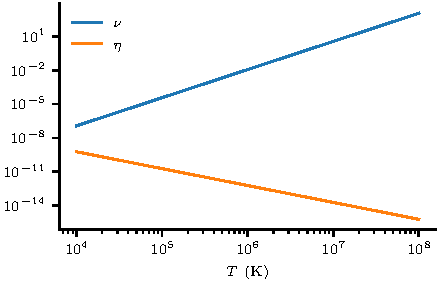
\includegraphics[width=0.5\linewidth]{visc_dep_on_temp.pdf}
  \mycaption{Dependence of non-dimensionalised viscosity $\nu$ and Spitzer resistivity $\eta$ on temperature.}{These are non-dimensionalised using typical coronal values of a magnetic field strength of $B = 5$ mT, a length of $L = 1$ Mm and a density of $\rho = 1.67 \times 10^{-12}$ kg m$^{-3}$. In the non-dimensionalisation scheme used here, the Reynolds and Lundquist numbers are the inverses of $\nu$ and $\eta$, respectively.}
  \label{fig:visc_dep_on_temp}
\end{figure}

The dominant mechanism of heat dissipation in the solar corona remains unknown, although Ohmic heating and viscous heating are two highly studied candidates. The transport parameters for viscosity $\nu$ and Spitzer resistivity $\eta$ can be derived by kinetic means as
\begin{equation}
  \label{eq:nu_and_eta}
\nu_{dim} = 10^{-17}\ T^{5/2} \text{ kg m}^{-1}\text{ s}^{-1}, \quad \eta_{dim} = 2\times 10^{9}\ T^{-3/2}\ \text{ m}^2 \text{ s}^{-1},
\end{equation}
where $T$ is the plasma temperature in Kelvin. Both expressions are taken from~\cite{braginskiiTransportProcessesPlasma1965}. Non-dimensionalising these using the scheme found in~\cite{arberStaggeredGridLagrangian2001} and typical coronal values for the Alfv\'en velocity $v_A = 3.45 \times 10^6$ m s$^{-1}$, length scale $L_0 = 1$ Mm and density $\rho_0 = 1.67 \times 10^{-12}$ kg m$^3$ give
\begin{equation}
  \label{eq:nondim_nu_and_eta}
\nu = 1.6 \times 10^{-18}\ T^{5/2} \quad \eta = 5.8 \times 10^{-4}\ T^{-3/2}.
\end{equation}
Using this non-dimensionalisation scheme the Reynolds number is given $Re = 1/\nu$ and the Lundquist number $S = 1/\eta$. Figure~\ref{fig:visc_dep_on_temp} shows the dependences of the non-dimensionalised $\nu$ and $\eta$ on temperature $T$. For a typical active region temperature of $T = 10^6$ K, $\nu \approx 10^{-3}$ and $\eta \approx 10^{-13}$.

Comparing the transport parameters for each dissipation mechanism suggests viscous heating should outperform Ohmic heating by several orders of magnitude. Indeed, many studies provide evidence to this effect~\cite{browningMechanismsSolarCoronal1991,craigViscousDissipation3D2013,craigAnisotropicViscousDissipation2009a,armstrongViscoResistiveDissipation2013,hollwegViscosityChewGoldbergerLowEquations1986a}. However, these parameters are unlikely to reflect the true degree of dissipation in the solar corona due to the influence of various effects which can enhance the effective dissipation beyond the values found via~\eqref{eq:nu_and_eta}. 

Turbulence can enhance viscosity~\cite{canutoTurbulentViscosity1988} and many mechanisms for the anomalous enhancement of resistivity have been suggested, including turbulence~\cite{cheHowAnomalousResistivity2017} and the impact of electron scattering~\cite{maEffectiveResistivityCollisionless2018}. The degree to which either dissipation mechanism is enhanced in the solar corona is difficult to estimate, however some studies have attempted to infer the effective transport parameters from observations of wave motions in coronal loops~\cite{nakariakovTRACEObservationDamped1999}, although results are disputed~\cite{klimchukCoronalSeismologyPropagation2004}. A further complication in attempting to model dissipation in the solar corona is that it is still unknown how far the collisional approximation holds~\cite{klimchukSolvingCoronalHeating2006a}.

Due to numerical diffusion present in any numerical scheme~\cite{ferzigerComputationalMethodsFluid2002}, state of the art, 3D numerical experiments are only able to probe diffusion parameters down to approximately $10^{-5}$ (non-dimensional). While this theoretically reaches the bounds of realistic viscosity, it is not close to even enhanced estimates of resistivity. Until numerical techniques and computational resources become sophisticated enough to probe realistic (enhanced or otherwise) dissipation parameters, the true nature of dissipation in the solar corona remains unclear. At best, the community can infer the importance of these and other dissipation mechanisms by constructing scaling laws for computationally feasible parameters, as is done in~\cite{craigViscousDissipation3D2013}.

\section{MHD Equations}

\subsection{The Navier-Stokes equations}

The Navier-Stokes equations are a set of partial differential equations (PDEs) which model the dynamics of a fluid through conservation of mass, momentum and energy. Generally, the equations are derived by considering conservation of the relevant quantity in a small parcel of fluid that moves with the flow. Such a derivation may be found in, for example~\cite{andersonComputationalFluidDynamics1995}. In the following description of the equations, use is made of the material derivative
\begin{equation}
  \label{eq:material_derivative}
  \frac{D}{Dt} \equiv \frac{\partial}{\partial t} + (\vec{u} \cdot \nabla)
\end{equation}
which describes the change in a quantity as it moves with flow at a velocity $\vec{u}$.

Modelling conservation of mass, the continuity equation describes the change in density $\rho$ due to the compression or dilation of the flow,
\begin{equation}
\frac{D\rho}{Dt} = - \rho \vec{\nabla} \cdot \vec{u}.
\label{eq:ns_continuity}
\end{equation}
The momentum equation is an application of Newton's second law and models the conservation of momentum in a fluid with a scalar thermal pressure $p$ and viscous stress tensor $\ten{\sigma}$,
\begin{equation}
\rho\frac{D\vec{u}}{Dt} = -\vec{\nabla} p + \vec{\nabla} \cdot \ten{\sigma}.
\label{eq:ns_momentum}
\end{equation}
The energy equation is given as
\begin{equation}
\rho\frac{D\varepsilon}{Dt} = -p \vec{\nabla} \cdot \vec{u} + \ten{\sigma} : \vec{\nabla}\vec{u},
\label{eq:ns_energy}
\end{equation}
and describes the change in internal thermal energy due to work done by pressure and viscous heating. Here, the double dot product (or tensor double contraction) is defined as $\ten{A}:\ten{B} = A_{ji} B_{ij}$ for arbitrary tensors $\ten{A}$ and $\ten{B}$. This system of equations must be closed by an additional equation of state. As presented later, the ideal equation of state is sufficient, for the purposes of describing coronal plasma.

While the Navier-Stokes equations adequately describe many fluids, conducting fluids like ionised plasmas and liquid metals couple with local magnetic fields and require an extension to the governing equations. The result are the equations of magnetohydrodynamics.

\subsection{Magnetohydrodynamics and the induction equation}

Magnetohydrodynamics (MHD) describes electrically conducting fluids, that is fluids which interact with electromagnetic fields. Typical examples of such fluids are ionised plasmas and molten metals, the investigation of the latter being key to the understanding of the Earth's molten outer core and its associated magnetic dynamo. Both small-scale laboratory plasmas, such as those found in current fusion devices, and large-scale astrophysical plasmas, such as those in the interstellar medium, can be effectively modelled using the MHD equations. While these equations have a large range of applicability, they are limited to systems with dynamics at length scales much larger than the ion skin depth or Larmor radius, and time scales much longer than the ion gyration time. For systems where the length or time scales are too small to be described by MHD, a kinetic approach using, for example, the Vlasov or Boltzmann equations is more appropriate. The ideal MHD equations can be recovered from the Boltzmann equation by taking appropriate moments~\cite{boydPhysicsPlasmas2003}.

The MHD equations are a synthesis of the Navier-Stokes equations of fluid dynamics and Maxwell's equations of electromagnetism. The latter set of equations describes the generation of an electric field $\vec{E}$ by a charge density $\rho_c$ through Gauss's law,
\begin{equation}
  \label{eq:gauss_law}
 \nabla \cdot \vec {E} ={\frac {\rho_c }{\varepsilon _{0}}},
\end{equation}
the non-existence of monopoles in the magnetic field $\vec{B}$,
\begin{equation}
  \label{eq:gauss_law_for_magnetism}
  \nabla \cdot \vec {B} =0,
\end{equation}
the generation of electric fields due to changes in the magnetic field in time $t$ through the Maxwell-Faraday equation,
\begin{equation}
  \label{eq:maxwell_faraday}
 \nabla \times \vec {E} =-{\frac {\partial \vec {B} }{\partial t}},
\end{equation}
and the generation of magnetic fields due to currents $\vec{\jmath}$ and changing electric fields through Ampère's law,
\begin{equation}
  \label{eq:ampere_law}
 \nabla \times \vec {B} =\mu _{0}\left(\vec {\jmath} +\varepsilon _{0}{\frac {\partial \vec {E} }{\partial t}}\right).
\end{equation}
Written in SI units, these equations use the permittivity $\varepsilon_{0}$ and permeability $\mu_0$ of free space.

Many conducting fluids can be considered electrically neutral, that is on the timescale of fluid motion the charges within the fluid are able to quickly redistribute to nullify any electric forces. This is true for coronal plasmas where the electrons, being much lighter than the ions, are free to quickly redistribute imbalances in charge density. This allows Gauss's law to be entirely neglected. The displacement current, the last term in Ampère's law, can also be neglected using the assumption that fluid motions are non-relativistic, that is the typical fluid velocity is much less than the speed of light, $c$~\cite{priestMagnetohydrodynamicsSuna}.

In order to couple the fluid motion to the electromagnetic fields, a constitutive Ohm's law is also included which describes the generation of currents in response to electric fields. This eventually allows the complete elimination of $\vec{E}$ from the governing equations. In a fluid's rest frame, the current response to an electric field $\vec{E}'$ is
\begin{equation}
  \label{eq:rest_frame_ohms_law}
  \vec{\jmath} = \sigma \vec{E}',
\end{equation}
where $\sigma$ is the (finite) conductivity of the fluid. The Lorentz transformation to the frame where the fluid is moving at velocity $\vec{u}$ is
\begin{equation}
  \label{eq:resistive_ohms_law}
  {\vec {E}}+{\vec{u}}\times {\vec {B}}=\eta{\vec {\jmath}},
\end{equation}
where the conductivity has been rewritten as the resistivity $\eta = 1/\sigma$. In the case of perfect conductivity, Ohm's law is written
\begin{equation}
  \label{eq:ideal_ohms_law}
  {\vec {E}}+{\vec{u}}\times {\vec {B}}=0.
\end{equation}
Additional non-ideal physics like ambipolar diffusion and the Hall effect can be modelled through additional terms in Ohm's law. However, in the solar corona these effects are small compared to resistivity and are neglected here~\cite{priestMagnetohydrodynamicsSuna}.

Combining the remaining parts of Ampère's law, the Maxwell-Faraday equation, and the resistive Ohm's law results in the induction equation,
\begin{equation}
  \label{eq:nonsimple_induction_equation}
{\frac {\partial \vec {B} }{\partial t}} = \nabla \times (\vec{u} \times \vec{B}) - \nabla \times (\eta/\mu_0 \nabla \times \vec{B}),
\end{equation}
which, in the case of uniform resistivity, may be written
\begin{equation}
  \label{eq:induction_equation}
{\frac {\partial \vec {B} }{\partial t}} = \nabla \times (\vec{u} \times \vec{B}) + \frac{\eta}{\mu_0}\nabla^2 \vec{B}.
\end{equation}
This equation essentially describes the advection and generation of a magnetic field due to fluid motions and the diffusion of the field due to resistivity. The magnetic field must still satisfy the solenoidal constraint $\nabla \cdot \vec{B} = 0$.

In order to describe the effect of the magnetic field on the fluid, additional terms must be added to the momentum~\eqref{eq:ns_momentum} and energy~\eqref{eq:ns_energy} equations. The Lorentz force describes the force exerted by the magnetic field on the fluid and is given by
\begin{equation}
  \label{eq:lorentz_force}
\vec{\jmath} \times \vec{B}.
\end{equation}
When the fluid is resistive, the dissipation of currents can heat the fluid through a process called Joule or Ohmic heating. This is modelled in the energy equation by the term
\begin{equation}
\mu_0 \eta | \vec{\jmath} |^2.
\end{equation}

\subsection{The non-dimensionalised MHD equations}

\label{sec:mhd_equations}

Combining the fluid equations~\eqref{eq:ns_continuity}--\eqref{eq:ns_energy} and the induction equation~\eqref{eq:induction_equation}, the full set of MHD equations can be written in their non-dimensionalised form
\begin{gather}
%\begin{equation}
\label{eq:mhda}
\frac{D\rho}{Dt} = - \rho \vec{\nabla} \cdot \vec{u},\\
%\end{equation}
%\begin{equation}
\rho\frac{D\vec{u}}{Dt} = -\vec{\nabla} p + \vec{\jmath} \times \vec{B} + \vec{\nabla} \cdot \ten{\sigma},\\
%\end{equation}
%\begin{equation}
\frac{D\vec{B}}{Dt} = (\vec{B} \cdot \vec{\nabla})\vec{u} - (\vec{\nabla} \cdot \vec{u})\vec{B} + \eta \nabla^2 \vec{B},\\
%\end{equation}
%\begin{equation}
\rho\frac{D\varepsilon}{Dt} = -p \vec{\nabla} \cdot \vec{u} + {Q}_{\nu} + {Q}_{\eta},%\\
\label{eq:energy}
%\end{equation}
\end{gather}
where $\eta = 1/S$ is now the non-dimensionalised resistivity, equivalent
to the inverse of the Lundquist number $S$. This notation is used throughout the remainder of this thesis. The system is closed by the inclusion of the equation of state for an ideal gas
\begin{equation}
\varepsilon = \frac{p}{\rho(\gamma - 1)},
\end{equation}
where the specific heat ratio is given by $\gamma = 5/3$. The
  terms ${Q}_{\nu} = \ten{\sigma} : \vec{\nabla}\vec{u}$ and
  ${Q}_{\eta} = \eta | \vec{\jmath} |^2$ are viscous heating and Ohmic heating, respectively.

The non-dimensionalisation scheme is identical to that used in the code Lare3d~\cite{arberStaggeredGridLagrangian2001}, where a typical magnetic field strength $B_0$, density $\rho_0$ and length scale $L_0$ are chosen and the other variables non-dimensionalised appropriately. Velocity and time are
non-dimensionalised using the Alfv\'en speed $u_A = B_0 / \sqrt{\rho_0
  \mu_0}$ and Alfv\'en crossing time $t_A = L_0/u_A$,
respectively. Temperature is non-dimensionalised via $T_0 = u_A^2
\bar{m} / k_B$, where $k_B$ is the Boltzmann constant and $\bar{m}$ is
the average mass of ions, here taken to be $\bar{m} = 1.2m_p$ (a mass
typical for the solar corona) where $m_p$ is the proton mass. Dimensional quantities can be recovered by multiplying the non-dimensional variables by their respective reference value (e.g. $\vec{B}_{\dim} = B_0 \vec{B}$). All further reference to variables will be to their non-dimensionalised values, unless stated otherwise.

\section{Anisotropic Viscosity}

Viscosity plays an important part generally in astrophysical fluid dynamics. Recent studies have demonstrated the importance of anisotropic viscosity in coronal heating in investigations of three-dimensional (3D) null points~\cite{craigViscousDissipation3D2013}, current sheet merging~\cite{armstrongViscoResistiveDissipation2013} and flux pile-up~\cite{litvinenkoViscousEnergyDissipation2005}. There is further evidence of the importance of anisotropic viscosity in other astrophysical applications including the intracluster medium~\cite{zuhoneEffectAnisotropicViscosity2014, parrishEffectsAnisotropicViscosity2012a} and the solar wind~\cite{baleMagneticFluctuationPower2009}. In other solar applications, viscosity has a role to play in the damping of coronal instabilities~\cite{howsonEffectsResistivityViscosity2017} and waves~\cite{vranjesViscosityEffectsWaves2014, erdelyiResonantAbsorptionAlfven1995a, rudermanSlowSurfaceWave2000a}, though not all these cases have been fully explored using an anisotropic model of viscosity.

\subsection{Viscosity}

Physically, viscosity is the internal friction of a fluid arising due to interactions (typically collisions) between the particles making up the fluid. Within the context of MHD, viscosity provides two functions. The first is momentum transport, included in the momentum equation as the divergence of the viscous stress tensor $\ten{\sigma}$, written using Einstein notation as
\begin{equation}
  \label{eq:viscous_momenum_transport}
  (\nabla \cdot \ten{\sigma})_j = \frac{\partial \sigma_{ij}}{\partial x_i}.
\end{equation}

In three dimensions, the nine components of $\ten{\sigma}$ quantify the flux of each component of momentum in each direction of motion as a result of viscous diffusion. For example, the $\sigma_{xy}$ component gives the flow of $x$-momentum in the $y$-direction. Due to symmetry arising from viscosity conserving angular momentum, the tensor is symmetric, so the component $\sigma_{xy}$ also quantifies the flux of $y$-momentum in the $x$-direction. Beyond the requirement of conservation of angular momentum, it is also assumed that Stokes' hypothesis holds, that is bulk viscosity is zero and viscosity does not act under uniform compression or expansion of the fluid. This requires the viscous stress tensor to be additionally trace-free,
\begin{equation}
  \label{eq:trace_free_tensor}
  \text{tr}(\ten{\sigma}) = 0.
\end{equation}
Due to the viscous stress tensor being trace-free and symmetric, the number of independent components reduces from nine to five.

The second function of viscosity is to convert kinetic into thermal energy through work done by local deformations. This is encoded in a term in the energy equation of the MHD equations of the form
\begin{equation}
  \label{eq:viscous_heat_generation}
  \ten{\sigma} : \nabla \vec{u} = \sigma_{ij} \frac{\partial u_i}{\partial x_j},
\end{equation}
and may also be written using the rate of strain tensor $\ten{W}$ as
\begin{equation}
  \label{eq:viscous_heat_generation2}
  \ten{\sigma} : \nabla \vec{u} = \frac{1}{2} \ten{\sigma} : \ten{W},
\end{equation}
where
\begin{equation}
  \label{eq:rate_of_strain}
  \ten{W} = \nabla\vec{u} + (\nabla\vec{u})^T - \tfrac{2}{3}(\nabla \cdot \vec{u})\ten{I}.
\end{equation}
The tensor $\ten{W}$ quantifies the rate at which a parcel of fluid undergoes a deformation and is symmetric and trace-free by construction.

Many fluids encountered in nature are Newtonian fluids, that is the viscous stress arising from any deformation of the fluid is directly proportional to the rate of strain of the deformation,
\begin{equation}
  \label{eq:isotropic_viscous_tensor}
  \ten{\sigma} = \nu \ten{W},
\end{equation}
where $\nu$ is the viscous transport parameter, generally referred to as the viscosity. However, in a magnetised plasma the nature of particle collisions is distinctly different from those in a non-conducting fluid and the nature of viscosity different as a result.

\subsection{Viscosity in a magnetised plasma}

\label{sec:visc_in_magnetised_plasma}

In a Newtonian fluid, the motion of a single particle travelling with typical thermal velocity $v$ and colliding with other particles in a typical collision time $\tau$ will appear as a number of broken, straight lines, each of approximate length $l = v\tau$, where $l$ is the mean free path. These motions have no preferred direction resulting in an isotropic transfer of momentum. In contrast, in a plasma made up of charged particles with charge $e$ and mass $m$, threaded by a magnetic field of strength $B$, the particles follow helical paths of approximate radius $r = v/\omega$, where $\omega = eB/m$ is the cyclotron frequency. After a time $\tau$, a typical particle will undergo a collision and its path will describe a new helix. The total resultant motion depends on the strength of the magnetic field. In the presence of a weak field, the radius of the helix may be much larger than the mean free path or in terms of the cyclotron frequency, $\omega \tau \ll 1$. As a result, the path between collisions will be close to straight and the total path will resemble that of the motion without a magnetic field. In the presence of a strong field, $\omega \tau \gg 1$ and a typical particle will be able to wind around the field a number of times, travelling a distance $l$ along the field, before colliding. As a result the transport of momentum is strongly anisotropic to the extent that it is unaffected in the direction of the field, but strongly reduced in the transverse direction.

A characteristic coronal value of $\omega \tau$ can be calculated using expressions found in Braginskii~\cite{braginskiiTransportProcessesPlasma1965}. The collision time can be written in SI units as
\begin{equation}
  \label{eq:collision_time}
  \tau = 0.82 \times 10^{-6} \frac{T^{3/2}}{n} \text{ s},
\end{equation}
where $n$ is the number density. The cyclotron frequency is written as
\begin{equation}
  \label{eq:cyclotron_frequency}
  \omega = 0.96\times10^8 B \text{ s}^{-1},
\end{equation}
where the Coloumb logarithm has been taken to be 22, and the mass fraction, the ratio of ion to proton mass, $m_f = m_i/m_p$ has been taken to be a typical solar value of $1.2$. A solar active region has typical temperatures of around $2\times 10^6$ K and number densities of $n = 3 \times 10^3\text{ m}^{-3}$, giving $\tau = 0.773$ s. The magnetic field can be as strong as $5\times 10^{-3}$ T, giving $\omega = 4.79 \times 10^5 \text{ s}^{-1}$, resulting in $\omega \tau = 3.70 \times 10^5$. Even in the quiet sun, $\omega\tau \approx 10^4$~\cite{morganGlobalConditionsSolar2017}. This indicates viscosity in most of the solar corona is highly anisotropic. 

\subsection{Anisotropic viscous tensors}

The form of the viscous stress tensor in a magnetized plasma has been derived in a number of ways to varying degrees of accuracy. The derivations typically use the methods of kinetic theory, taking moments of the Boltzmann-Maxwell equations to arrive at continuum-level approximations of the stress tensor.

A first approximation of the stress tensor can be found in the work of Chapman and Cowling~\cite{chapmanMathematicalTheoryNonuniform1970}. Their results show that the stress response to a rate of strain can be considered as responses to three types of deformation: compression or dilation along the field, deformations in the plane transverse to the field, and deformations in the plane including the field. The foremost deformation gives rise to the parallel component of viscosity, typically the largest in magnitude and often the only component modelled in applications~\cite{parrishEffectsAnisotropicViscosity2012a}. The latter two deformations give rise to two stress responses each, totalling four components: two perpendicular components and two drift components. In total there are five contributions to the viscous stress tensor in a magnetised plasma, each with an associated transport parameter. The reader is directed to a discussion by Kaufman~\cite{kaufmanPlasmaViscosityMagnetic1960} where he presents both an illustrative description of the drift and perpendicular components of the tensor, and a derivation of the full tensor from a more simplified Boltzmann equation than is used in~\cite{chapmanMathematicalTheoryNonuniform1970}. The parallel component of the stress tensor has been derived without use of kinetic theory by Hollweg~\cite{hollwegViscosityMagnetizedPlasma1985}, showing that the viscous response to parallel motions is a result of collisions repartitioning anisotropies in the thermal pressure. The tensor derived by Braginskii~\cite{braginskiiTransportProcessesPlasma1965} is perhaps the most well known and includes accurate approximations of the five viscous transport parameters.

\subsection{Simplified derivation of Braginskii tensor}

This section presents a condensed version of Braginskii's qualitative derivation of the form of the anisotropic viscosity stress tensor in a magnetized plasma, and its associated transport parameters~\cite{braginskiiTransportProcessesPlasma1965}. 

Consider a plasma where, on average, each particle moves a distance $\Delta x$ in the collision time $\tau$ before colliding. After the collision the particle has equal probability of moving to the left or the right. Since we are concerned with the viscous diffusion of momentum, and not the advection of momentum, we consider the case where the net particle flux through the plane $x=x_0$ is zero, that is the number of particles moving through the plane from the left is equal to the number of particles from the right. This implies a uniform number density in the small layer around $x_0$.

Now consider a non-uniform velocity component $u$ which changes slowly enough over the distance $\Delta x$ that we may write
\begin{equation}
  \label{eq:viscous_derivation_vy}
u (x) \approx u(x_0) + \frac{\partial u}{\partial x} \bigg| _{x_0} (x - x_0).
\end{equation}

Within a time $\tau$ half the particles in the layer between $x_0 - \Delta x$ and $x_0$ will pass through the plane $x_0$, the other half moving in the opposite direction. The flux of momentum from the left is
\begin{equation}
  \label{eq:momentum_flux_left}
F_{+} = \frac{1}{2} \int^{x_0}_{x_0 - \Delta x} \frac{1}{\tau} m n u(x) \text{d}x = \frac{mn}{2} \left[ u(x_0) - \frac{\partial u}{\partial x} \frac{\Delta x}{2} \right] \frac{\Delta x}{\tau},
\end{equation}
and the flux from the right $F_{-}$ can be calculated in a similar manner by considering the flux from the layer between $x_0$ and $x_0 + \Delta x$. The total flux of momentum moving through the point $x_0$ is
\begin{equation}
  \label{eq:total_momentum_flux}
  F = F_+ - F_- = - \nu \frac{\partial u}{\partial x}, \quad \nu \sim \frac{nm(\Delta x)^2}{\tau}.
\end{equation}
The change in momentum at the point $x_0$ is then given by the negative slope of the momentum flux $- \partial F/\partial x$. Thus, the quantity $-F$ is a measure of one component of the viscous stress tensor $\ten{\sigma}$, with the overall strength of viscous dissipation governed by the parameter $\nu$. For example, if $u$ is the velocity in the $y$-direction, $-F$ estimates the value of $\sigma_{yx}$. Substituting $\Delta x$ for appropriate lengths in the expression for $\nu$ reveals the relative strengths of the viscous response to various motions. 

In the absence of a magnetic field the viscosity is isotropic and particles are able to travel the full mean free path before colliding, hence $\Delta x = u \tau$, where $u$ is the thermal velocity. This gives an estimate for the isotropic viscous response,
\begin{equation}
  \label{eq:isotropic_eta_estimate}
  \ten{\sigma}_{iso} \sim \eta_0 \ten{W}, \quad \eta_0 \sim nm\tau v^2 \sim nT \tau,
\end{equation}
where we use the notation $\eta_0 = \nu$ here to mirror Braginskii's derivation. This should not be confused with resistivity $\eta$.

Now consider a magnetic field aligned with the $z$-direction. A similar expression to that for isotropic viscosity is found when considering the viscous response to a field-aligned gradient in a field-aligned velocity $\partial u_z / \partial z$, where $\Delta x$ is still the mean free path,
\begin{equation}
  \label{eq:parallel_eta_estimate}
\sigma_{zz} \sim \eta_0 \frac{\partial u_z}{\partial z}.
\end{equation}
That is, in a magnetised plasma, compression or dilation along the field produces the same viscous response as if the field were not there.

Now consider the same velocity $u_z$ changing in a direction perpendicular to the field, say in the $x$-direction. Then $\Delta x$ is approximately the gyroradius $r = u/\omega$. The viscous response is then
\begin{equation}
  \label{eq:perp_eta_estimate}
\sigma_{zx} \sim \eta_{\perp} \frac{\partial u_z}{\partial x}, \quad \eta_{\perp} \sim \frac{\eta_0}{(\omega \tau)^2}.
\end{equation}
A similar expression holds when a velocity perpendicular to the field, say $u_y$, varies in the $x$-direction, that is
\begin{equation}
  \label{eq:perp_eta_estimate2}
\sigma_{xy} \sim \eta_{\perp} \frac{\partial u_y}{\partial x}.
\end{equation}

The viscous response to compression or dilation perpendicular to the field arises due to a different mechanism than the simple diffusion of momentum shown previously. When the plasma is compressed or dilated perpendicular to the field, the transverse energy of the particles changes and is subsequently equipartitioned by collisions. This takes place over a finite period of time, during which the transverse and longitudinal pressures differ. This difference in pressures gives rise to a stress of the same order as the parallel contribution
\begin{equation}
  \label{eq:compression_eta_estimate}
\sigma_{xx} = \sigma_{yy} \sim \eta_0 \nabla \cdot \vec{u}, \quad \sigma_{zz} \sim - \eta_0 \nabla \cdot \vec{u}.
\end{equation}

There are further contributions to the viscous stress tensor from motions which give rise to gyroviscous stresses, the transport parameters of which vary as $\eta_0 / (\omega \tau)$. As discussed later, these contributions produce no viscous heating and shall be neglected. For a detailed discussion of these terms, see~\cite{kaufmanPlasmaViscosityMagnetic1960}.

\subsection{The Braginskii tensor}

\label{sec:braginskii_tensor}

The full Braginskii viscous stress tensor can be written in a number of ways. Braginskii's original formulation is written with the magnetic field aligned with the $z$-axis so presented here is the more general formulation of Hogan~\cite{hoganCollisionalTransportMomentum1984}, described as the sum of five tensor components $\ten{W}^{(i)}$ with associated transport parameters $\eta_i$,
\begin{equation}
\label{eq:braginskii_tensor}
\ten{\sigma}_{\text{brag}} = \eta_0 \ten{W}^{(0)} + \eta_1 \ten{W}^{(1)} + \eta_2 \ten{W}^{(2)} - \eta_3 \ten{W}^{(3)} - \eta_4 \ten{W}^{(4)}.
\end{equation}

As discussed earlier, there are three types of motion that give rise to the five tensor components: compression or dilation along the field, deformations in the plane transverse to the field, and deformations in the plane including the field. The first type of motion gives rise to the parallel term,
\begin{equation}
  \label{eq:braginskii_parallel_term}
  \ten{W}^{(0)} = \frac{3}{2}(\ten{W}\vec{b}\cdot\vec{b}) \left( \vec{b} \otimes \vec{b} - \frac{1}{3}\ten{I} \right),
\end{equation}
where $\vec{b} = \vec{B}/|\vec{B}|$ is the unit vector in the direction of the field. The second and third types of motion give rise to two types of stress: two perpendicular terms,
\begin{align}
\ten{W}^{(1)} &= (\ten{I} - \vec{b} \otimes \vec{b})\ten{W}(\ten{I} - \vec{b} \otimes \vec{b}) + \frac{1}{2}(\ten{W}\vec{b} \cdot \vec{b})(\ten{I} - \vec{b} \otimes \vec{b}), \\
\ten{W}^{(2)} &= (\ten{I} - \vec{b} \otimes \vec{b})\ten{W}(\vec{b} \otimes \vec{b}) + (\vec{b} \otimes \vec{b})\ten{W}(\ten{I} - \vec{b} \otimes \vec{b}),
\end{align}
and two terms often called the drift or gyroviscous terms,
\begin{align}
\ten{W}^{(3)} &= \frac{1}{2} \ten{Z}\ten{W}(\ten{I} - \vec{b} \otimes \vec{b}) - \frac{1}{2}(\ten{I} - \vec{b} \otimes \vec{b})\ten{W}\ten{Z}, \\
\ten{W}^{(4)} &= (\ten{Z}\ten{W}\vec{b}) \otimes \vec{b} + \vec{b} \otimes (\ten{Z} \ten{W} \vec{b}),
\label{eq:drift_terms}
\end{align}
where the tensor $\ten{Z}$ has components $Z_{ij} = \varepsilon_{ikj}b_k$, where $\varepsilon_{ikj}$ is the Ricci alternating tensor (note the index ordering). It can be shown that these five tensors are mutually orthogonal, that is $\ten{W}^{(i)}:\ten{W}^{(j)} = 0$ for $i\ne j$.

Braginskii derives the five viscosity coefficients $\eta_i$ from a kinetic description of the plasma (see~\cite{epperleinPlasmaTransportCoefficients1986} for an example derivation). While more modern methods of deriving transport parameters have generally produced more accurate estimates~\cite{epperleinPlasmaTransportCoefficients1986}, Braginskii's expressions combine relative simplicity and good accuracy are are still widely used. These are the expressions used throughout this thesis.

The parallel viscosity coefficient $\eta_0$ is identical to the dynamic viscosity coefficient of an unmagnetised plasma $\nu$ and has already been given in expression~\eqref{eq:nu_and_eta}. For completeness, this is restated here,
\begin{equation}
\label{eq:nu}
\eta_0 = 0.68 \times 10^{-16} T^{5/2} \text{ kg m}^{-1} \text{ s}^{-1}.
\end{equation}

\begin{figure}[t]
  \centering
  \includegraphics[width=0.5\linewidth]{brag_coeffs.pdf}
  \mycaption{Dependence of Braginskii coefficients $\eta_1$ and $\eta_3$ on magnetic field strength.}{The collision time is $\tau = 0.77$ s, corresponding to a typical coronal temperature of $T=10^6$ K. Both expressions are normalised against $\eta_0$.}
\label{fig:visc_dep}%
\end{figure}

For simplicity, the dimensionless quantity $x = \omega \tau$ is used in the expressions for the remaining transport parameters, as is done in~\cite{braginskiiTransportProcessesPlasma1965}, and all coefficients have identical units to $\eta_0$. The two perpendicular coefficients are written,
\begin{equation}
  \label{eq:perp_visc_coeff}
  \eta_2(x) = \frac{\eta_0}{\Delta} \left( \tfrac{6}{5} x^2 + 2.23 \right), \quad \eta_1 = \eta_2(2x),
\end{equation}
where
\begin{equation}
  \label{eq:delta}
\Delta = x^4 + 4.03x^2 + 2.23.
\end{equation}
The drift coefficients are written,
\begin{equation}
  \label{eq:drift_visc_coeff}
  \eta_4(x) = \frac{\eta_0}{\Delta} x \left( x^2 + 2.38 \right), \quad \eta_3 = \eta_4(2x).
\end{equation}
The relative strength of the five coefficients is important in considering which are most significant in the solar corona. The drift coefficients are of the order $\eta_0/(\omega \tau)$ and the perpendicular coefficients of the order $\eta_0/(\omega \tau)^2$. The dependence on the magnetic field strength can be seen in figure~\ref{fig:visc_dep}.

As has already been discussed, the origin of each of the five viscosity components can be understood by considering the effect of velocity gradients and collisions on a plasma from a kinetic perspective. The drift terms are products of the velocity gradient perturbing particle orbits which generates pressure anisotropies and, in the absence of collisions, produces a stress which is orthogonal to the strain, resulting in no viscous dissipation. Collisions repartition the anisotropies in the pressure giving rise to the perpendicular terms. This is explored in detail by Kaufman in~\cite{kaufmanPlasmaViscosityMagnetic1960}. 

While it is illustrative to understand from a kinetic perspective why the drift terms produce no dissipation, it can be shown explicitly for the terms given in equation~\eqref{eq:drift_terms}. The strain rate tensor can be written as the sum of only the parallel and perpendicular terms, $\ten{W} = \ten{W}^{(0)} + \ten{W}^{(1)} + \ten{W}^{(2)}$. Since the drift terms are individually orthogonal to $\ten{W}^{(0)}$, $\ten{W}^{(1)}$ and $\ten{W}^{(2)}$, they are also orthogonal to $\ten{W}$. By equation~\eqref{eq:viscous_heat_generation2}, the drift terms cannot contribute to overall viscous dissipation. Furthermore, the relative size of the transport coefficients ($\eta_3 \propto \eta_0/(\omega\tau)$) suggests the drift terms may be completely neglected. While these terms can still meaningfully participate in certain dynamics~\cite{dellarPlanarChannelFlow2011,ferraroFiniteElementImplementation2006}, this thesis focuses on the impacts of viscosity on coronal heating and so the drift terms will be neglected throughout the remainder of this work. While a similar argument suggests the perpendicular terms should also be neglected ($\eta_1 \propto \eta_0/(\omega\tau)^2$), they are required to rewrite the Braginskii tensor in a form useful for numerical simulation, as discussed later.

\subsection{Limit of strong magnetic field}

As already mentioned, in an solar active region $\omega \tau \approx 10^5 \gg 1$ and the transport coefficients in equations~\eqref{eq:perp_visc_coeff} and~\eqref{eq:drift_visc_coeff} become negligibly small compared to the parallel coefficient. As a result, in the absence of any magnetic null points, the Braginskii tensor can be reduced to its strong-field approximation,
\begin{equation}
  \label{eq:strong_field_approx}
\ten{\sigma}_{\text{brag}} = \eta_0 \ten{W}^{(0)} = \tfrac{3}{2} \eta_0 (\ten{W} \vec{b} \cdot \vec{b}) ( \vec{b} \otimes \vec{b} - \tfrac{1}{3} \ten{I}).
\end{equation}
In a local coordinate system where the magnetic field is aligned with $\vec{e}_z$, the tensor is
\begin{equation}
  \label{eq:z_aligned_strong_field_approx}
\ten{\sigma}_{\text{brag}} = \tfrac{3}{2} \eta_0 W_{zz} ( \vec{e}_z \otimes \vec{e}_z - \tfrac{1}{3} \ten{I}),
\end{equation}
where $\vec{e}_z$ is the unit vector in the $z$-direction. Notice that the only velocity gradient to enter into the above tensor is that which is aligned with the magnetic field (including gradients stemming from the compressional $\nabla \cdot \vec{u}$ term in the rate of strain tensor, equation~\eqref{eq:rate_of_strain}). It can also be seen that the magnetic field has no effect on the component of viscosity parallel to the field; it is identical to the corresponding component in the isotropic stress tensor,
\begin{equation}
  \label{eq:z_aligned_iso}
  (\sigma_{\text{iso}})_{zz} = (\sigma_{\text{brag}})_{zz} = \eta_0 W_{zz}.
\end{equation}
In the strong-field regime, the only motion damped by viscosity is non-uniform compression or dilation of the plasma. 

This approximation is valid even for quiet Sun conditions, where $\omega\tau \approx 10^4$. Where this approximation fails is around magnetic null points, regions of the corona where the magnetic field vanishes. Null points are an important, abundant feature in the coronal magnetic field~\cite{edwardsNullPointDistribution2015} and participate in a number of important solar phenomena~\cite{massonNATUREFLARERIBBONS2009,moreno-insertisPLASMAJETSERUPTIONS2013,barnesRelationshipCoronalMagnetic2007}. Any general model of solar viscosity must go beyond the strong-field approximation and additionally incorporate viscosity in the limit of weak magnetic field.

\subsection{Limit of weak magnetic field}

While the full Braginskii tensor~\eqref{eq:braginskii_tensor} presents the natural separation of viscous responses into parallel, perpendicular and drift components, this form is unsuitable for numerical simulation when null points are present in the magnetic field. As the field strength goes to zero approaching a null point, the unit vector $\vec{b}$ in equations~\eqref{eq:braginskii_parallel_term}--\eqref{eq:drift_terms} becomes mathematically undefined. Numerically, the calculation of $\vec{b}$ involves division by the magnitude of the field which is a quantity close to or exactly zero near a null point, leading to errors or complete failure of the numerical scheme. Even if a numerical implementation were to check for a locally small field, it's unclear how the viscous terms and transport coefficients, as written in the form of equation~\eqref{eq:braginskii_tensor}, interact as the field strength tends to zero. By rewriting the tensor as
\begin{eqnarray}\label{eq:brag_new}
\ten{\sigma}_{\rm brag} = &&\frac{3\eta_0+\eta_1-4\eta_2}{2|\vec{B}|^4}(\ten{W}\vec{B}\cdot\vec{B})(\vec{B}\otimes\vec{B})\\
\nonumber
& &+~ \frac{\eta_1-\eta_0}{2|\vec{B}|^2}(\ten{W}\vec{B}\cdot\vec{B})\ten{I}\\
\nonumber
& &+~ \frac{\eta_2-\eta_1}{|\vec{B}|^2}[\ten{W}(\vec{B}\otimes\vec{B})+(\vec{B}\otimes\vec{B})\ten{W}] \\
\nonumber
& &+~ \eta_1\ten{W},
\end{eqnarray}
the anisotropic terms and isotropic term are clearly separated. The grouping of terms and the explicit use of $\vec{B}$ rather than $\vec{b}$ allows a numerical implementation to check the local value of $|\vec{B}|$ and, if it's smaller than some threshold, manually set the anisotropic coefficients in equation~\eqref{eq:brag_new} to zero, avoiding a division by $|\vec{B}|$.

Similar to the strong-field limit, it can be shown that the magnetic field in the weak-field limit has no effect on the field-aligned component of momentum transport in~\eqref{eq:brag_new}. That is, ~\eqref{eq:z_aligned_iso} still holds.

\section{Conclusion}

This chapter introduces the layers of the Sun, in particular the solar corona, and summarises some recent developments in coronal heating. The MHD equations are presented as a synthesis of the Navier-Stokes equations of fluid dynamics and Maxwell's equations of electromagnetism and are non-dimensionalised. Viscosity in a magnetised plasma is discussed in detail and the particular nature of viscosity in the solar corona is explored. This general introduction to the solar atmosphere provides the foundation upon which the remainder of the thesis is built.

\chapter{Application to the kink instability}
\label{chp:kink_instability}

\graphicspath{{images/kink_instability/}}

\section{Introduction}
\label{sec:kink_introduction}

In this chapter I investigate the effects of anisotropic viscosity on the kink instability~\cite{hoodKinkInstabilitySolar1979, hoodCoronalHeatingMagnetic2009}, believed to be a trigger for flares~\cite{srivastavaObservationKinkInstability2010} and an important mechanism in the theory of coronal heating through nanoflares~\cite{browningHeatingCoronaNanoflares2008a}. The instability has also been studied using shock viscosity~\cite{hoodCoronalHeatingMagnetic2009,barefordShockHeatingNumerical2015} but a detailed investigation of the effects of Newtonian and Braginskii viscosity has not, to the best of my knowledge, been performed. In particular, the main aim of this investigation is to provide insight into the effect of the choice of viscosity model on the nonlinear dynamics and relaxation of a twisted coronal loop, where the kink instability converts magnetic energy to heat through Ohmic heating generated via current structures and through viscous heating generated via flow structures. I aim to give an estimate of how well viscous heating (using both isotropic and anisotropic models) performs when compared with Ohmic heating. This study extends previous work~\cite{hoodCoronalHeatingMagnetic2009} which also considers the kink instability in a zero-current loop (details given below). However, in contrast to~\cite{hoodCoronalHeatingMagnetic2009}, only background resistivity and viscosity are used as the two mechanisms of heat generation (that is, shock viscosity and anomalous resistivity are disabled). This investigation also provides further validation of the switching model in a simpler topology to that used by MacTaggart et al.~\cite{mactaggartBraginskiiMagnetohydrodynamicsArbitrary2017}, simpler in that there are no null points present in the field at any time.

The layout of the chapter is as follows. The coronal loop model is described in Section~\ref{sec:model-setup}. Details of the numerical setup and methods used in the analysis of the simulation results are presented in Section~\ref{sec:general-numerical-setup}. Detailed numerical results of a typical case of a kink instability are given in Section~\ref{sec:results} with a particular focus on how the different viscosity models affect its nonlinear evolution. The results of the typical case are confirmed and generalised by a parameter study in Section~\ref{sec:results2} where the dependences of the Ohmic and the viscous heating on the resistivity and the dynamic viscosity are explored. Conclusions are summarised in Section~\ref{sec:conclusions}.

This chapter is an adaptation of a previously published paper~\cite{quinnEffectAnisotropicViscosity2020a}. 

\section{Coronal loop model}
\label{sec:model-setup}

A twisted magnetic flux rope is used as the model of an idealised coronal loop. The domain is a Cartesian box of dimension $[-2\text{ Mm},2\text{ Mm}] \times [-2\text{ Mm},2\text{ Mm}] \times [-10\text{ Mm},10\text{ Mm}]$ in the $x$, $y$ and $z$-directions, respectively. The state of the plasma is typical of the corona, with density $\rho$ initially $1.67\times 10^{-12} \text{ kg m}^{-3}$, and with plasma pressure $p$ such that the temperature of the plasma $T$ is initially $2\times10^{4} \text{ K}$ everywhere in the domain. The magnetic field $\vec{B}$ is constructed so that it is initially force-free and with zero axial current, line-tied at the boundaries, and twisted such that it is linearly unstable to the ideal kink instability. This configuration allows direct comparison to previous studies that use similar magnetic field configurations~\cite{hoodCoronalHeatingMagnetic2009,barefordShockHeatingNumerical2015,bothaObservationalSignaturesCoronal2012}. The field outside the flux tube is straight and has a strength of $5\times10^{-3} \text{ T}$. Given this temperature and magnetic field strength, the plasma beta is initially $\beta \approx 10^{-5}$, a value realistic for the corona. The evolution of this flux tube is governed by the nonlinear MHD equations described in section~\ref{sec:mhd_equations}.

\begin{table}[t]
\centering
\begin{tabular}{ccc|ccc}
$B_0$ & $L_0$ & $\rho_0$ & $u_A = B_0 / \sqrt{\rho_0 \mu_0}$ & $t_A = L_0/u_A$ & $T_0$ \\ \midrule
$5 \times 10^{-3} \ \text{T}$ & $1\ \text{Mm}$ & $1.67 \times 10^{-12} \ \text{kgm}^{-3}$ & $3.45\ \text{Mms}^{-1}$ & $0.29\ \text{s}$ & $1.73 \times 10^{9}K$\\
\end{tabular}
\caption{Reference values for the magnetic field, length, density, and
  temperature. These are used to non-dimensionalise the MHD
  equations \eqref{eq:mhda}--\eqref{eq:energy} and to calculate the reference values for velocity, time and temperature.}
\label{tab:reference-values}
\end{table}

The magnetic field is considered force-free, that is the field is constructed such that the Lorentz force is zero, or $(\nabla \times \vec{B})\times \vec{B} = 0$. In cylindrical coordinates $(r,\theta,z)$, the chosen force-free magnetic field takes the form $\nabla \times \vec{B} = \alpha(r)\vec{B}$, where $\alpha(r)$ is a function of a particular form that ensures the total axial current is zero. Aligning with previous work by Hood et al.~\cite{hoodCoronalHeatingMagnetic2009}, the smooth $\alpha(r)$ profile given as Case 3 in~\cite{hoodCoronalHeatingMagnetic2009} is used. Using this profile, the equilibrium magnetic field $\vec{B}$ is written as 
\begin{equation}
\begin{aligned}
  \label{eq:field-profile-r-lt-1}
  B_{\theta} &= \lambda r {(1 - r^2)}^3,\\
  B_z &= \sqrt{1 - \frac{\lambda^2}{7} + \frac{\lambda^2}{7}{(1 - r^2)}^7 - \lambda^2 r^2 {(1-r^2)}^6},\\
  \alpha(r) &= \frac{2 \lambda {(1-r^2)}^2 {(1-4r^2)}}{B_z},
\end{aligned}
\end{equation}
for $r \leq 1$ and
\begin{equation}
\begin{aligned}
  \label{eq:field-profile-r-gt-1}
  B_{\theta} &= 0 \\
  B_z &= \sqrt{1 - \frac{\lambda^2}{7}}\\
  \alpha(r) &= 0 ,
\end{aligned}
\end{equation}
for $r > 1$, where $\lambda$ is a parameter measuring the twist in the tube. The radial field throughout the domain is set to $B_r = 0$. As is done in~\cite{hoodCoronalHeatingMagnetic2009}, $\lambda = 1.8$ to ensure the tube is unstable to the ideal kink instability. The equilibrium velocity for this magnetic field configuration is $\vec{u} = \vec{0}$.

\begin{figure}[t]
  \centering
  \begin{subfigure}[b]{0.48\textwidth}
  \begin{center}
    \begin{overpic}[width=\textwidth]{field_line_plots/cropped/v1e-4r5e-4.5-isotropic_0000_cropped.png}
      \put (50,5) {\small\textbf{(a)}}
    \end{overpic}
  \end{center}
  \end{subfigure}
  \begin{subfigure}[b]{0.48\textwidth}
  \begin{center}
    \begin{overpic}[width=\textwidth]{alpha_profile.pdf}
      \put (47,54) {\small\textbf{(b)}}
    \end{overpic}
  \end{center}
  \end{subfigure}
  \caption{\textit{The initial field configuration.} In \textbf{(a)} field lines are plotted corresponding to inner (red), outer (blue) and straight (yellow) regions of twist, with slices of $\alpha(r)$ shown at the footpoints. In the slices, red corresponds to $\alpha(r) > 0$, blue to $\alpha(r) < 0$ and white to $\alpha(r) = 0$. In \textbf{(b)} the profiles of $\alpha(r)$ and the field components $B_z$ and $B_{\theta}$ across the flux tube are plotted.}
\label{fig:field_configuration}
\end{figure}

The form of $\alpha(r)$ in equations~\eqref{eq:field-profile-r-lt-1} and~\eqref{eq:field-profile-r-gt-1} splits the profile of the flux tube into three twist regions, the inner region of positive twist ($r\le0.5$), the outer region of negative twist ($0.5<r<1$) and the straight-field region of zero twist ($r\ge1$) as shown in Figures~\ref{fig:field_configuration}(a) and (b). These figures also illustrate the equilibrium field. Since the inner region is more tightly twisted, this field configuration results in only the inner region becoming unstable to the kink instability, rather than the global instability seen in non-zero-current loops~\cite{hoodKinkInstabilitySolar1979}. The regions of twist are used later to define a measure of reconnection.

Although the initial temperature is prescribed as $T=2\times10^{4} \text{ K}$, the equations simulated by the code are written using internal energy, thus the temperature is converted to internal energy using the non-dimensional relation $\varepsilon = T/(1-\gamma)$. Hence, the initial non-dimensionalised density and internal energy are uniformly given by
\begin{equation}
  \rho = 1,\quad \varepsilon = 8.66 \times 10^{-4},
\end{equation}
and have been non-dimensionalised using the reference values found in Table~\ref{tab:reference-values}. The initial magnetic field and velocity are set to their equilibrium states, discussed above, with the addition of a small perturbation.

In order to make a meaningful comparison of the following results with those of~\cite{hoodCoronalHeatingMagnetic2009}, identical initial magnetic field and velocity perturbations are used, calculated via a linear stability analysis (in ideal MHD) applied to a similar flux tube that uses a constant, piecewise profile for $\alpha(r)$~\cite{vanderlindenCompleteCoronalLoop1999,browningSolarCoronalHeating2003c,browningHeatingCoronaNanoflares2008a}.

At the boundaries, the line-tied condition on the magnetic field is satisfied by ensuring the field is constant and equal to its initial values given by equations~\eqref{eq:field-profile-r-lt-1} and~\eqref{eq:field-profile-r-gt-1}. Similarly, on the boundaries the density, internal energy and velocity $\vec{u}$ are considered constant and equal to their initial values. To close the system, the fluxes of all variables through each of the boundaries are set to zero. That is, on the $x$-boundary,
\begin{equation}
  \frac{\partial \vec{B}}{\partial x} = \frac{\partial \vec{u}}{\partial x} = \vec{0}; \quad \frac{\partial \rho}{\partial x} = \frac{\partial \varepsilon}{\partial x} = 0 \quad \text{for } x=\pm 2,
\end{equation}
and similarly, the $y$ and $z$ derivatives are zero on the $y=\pm2$ and $z=\pm10$ boundaries, respectively.

Since there are no nulls created during the evolution of the kink instability, the field remains strong everywhere and the viscosity reverts to fully parallel. To ensure this, the switching model~\ref{eq:switching_model} is used with the von Mises switching function~\ref{eq:switching_function} where $a_0 = 150$. 

\section{Methods}
\label{sec:general-numerical-setup}

In this section the parameters of the numerical setup is presented, and various tools and quantities used in the proceeding analysis are described.

\subsection{Numerical setup}

The MHD equations~\eqref{eq:mhda}---\eqref{eq:energy} were solved numerically using the Lare3d code~\cite{arberStaggeredGridLagrangian2001}, previously described in chapter~\ref{chp:numerical_methods}. Shock viscosity was disabled in order to properly investigate the effect of different viscosity models. In order to compare results with those of Hood et al.~\cite{hoodCoronalHeatingMagnetic2009} numerical tests were performed using shock viscosity instead of either the switching or isotropic models. Using the default shock viscosity parameters present in the code, the behaviour closely mirrors that of isotropic viscosity with $\nu\approx 5\times10^{-4}$. When both switching and shock viscosity are enabled, the shock viscosity dominates and, again, the behaviour mirrors that of isotropic viscosity.

The simulations were run at a resolution of $350 \times 350 \times 700$, with the exception of the parameter studies, which were run at a slightly higher resolution of $400 \times 400 \times 800$. Since the switching viscosity only acts parallel to the magnetic field, in perpendicular directions numerical diffusion dominates. By running several simulations at resolutions of $250 \times 250 \times 500$ up to $500 \times 500 \times 1000$, it was found that the effect of resolution was negligibly small until around $t=150$, well after the nonlinear phase of the instability. After this time there were some quantitative differences in outputs for different resolutions. However, the qualitative behaviour, described later, does not strongly depend on the resolution.

The numerical diffusion present in the simulations (due to the finite difference scheme employed in Lare3d) is estimated as $\tilde{\nu} = \tilde{\eta} = \tilde{u}_x L_x/N_x^2$. Taking a typical velocity of $\tilde{u}_x = 1$, i.e.\ the Alfv\'en velocity; $N_x = 350$ as the number of grid-points in the $x$-direction; and $L_x = 4$ as the length in the $x$ direction, the numerical diffusion coefficient is estimated as $\tilde{\nu} = \tilde{\eta} \approx 10^{-5}$. This provides a theoretical lower bound on simulating a physical viscosity or resistivity. In practice, setting the physical resistivity lower than $\eta \approx 5\times10^{-5}$ results in behaviour that does not converge with increasing resolution. This gives a practical lower bound for diffusion coefficients of $\tilde{\nu} = \tilde{\eta} \approx 5 \times 10^{-5}$. Thus, all results presented use physical diffusion coefficients (either viscosity or resistivity) greater than this lower bound.

\subsection{Methods of analysis}

\subsubsection{Connectivity}

The mean change in field line connectivity $\Delta\Phi_c$ is used as a practical measure of reconnection rate. The connectivity of a given field line $\Phi_c$ is determined by comparing its start and end points. Any field line that begins at one location in one of the loop footpoints will map to a corresponding point in the opposite footpoint. Following field lines from their starting point at $z=-10$ to their end point at $z=10$, lines are labelled depending on the twist regions in which they start and end. Initially, the field lines within each distinct region map one-to-one to the same region. As the field reconnects radially during the instability, field lines begin to start and end in different twist zones. The rate of reconnection is estimated by tracking the number of field lines that have changed twist zones within a set time period. This also serves as a visual representation of where such reconnection is occurring. It should be noted that this measure of reconnection does not take into account azimuthal reconnection (that is reconnection within the same twist zone). As such, it is only a partial measure of reconnection.

In practice, magnetic field output is saved from the code at intervals of $\Delta t = 5$. The visualisation tool Mayavi~\cite{ramachandran2011mayavi} is used to compute the magnetic field lines over a grid of starting points $(x_i, y_j)$ at a given time $n \Delta t$, where $n$ indexes the output files. This process gives a connectivity map $\Phi_c^{(n)}(x_i, y_j)$ across the profile of the flux tube. The mean difference in connectivity $\Delta \Phi_c^{(n)}$ at time $n\Delta t$ is found by subtracting one connectivity map from the previous and then taking the mean across all points $(x_i, y_j)$,
\begin{equation}
  \Delta \Phi_c^{(n)} = \frac{1}{N_x N_y} \sum_{i=1}^{N_x} \sum_{j=1}^{N_y} (\Phi_c^{(n)}(x_i, y_j) - \Phi_c^{(n-1)}(x_i, y_j)).
\end{equation}

\subsubsection{Parallel electric field}

Another useful measure of magnetic reconnection is the maximum value of the integral of the electric field parallel to the magnetic field $E_{\parallel} = \eta {(\vec{\jmath} \cdot \vec{B})}/|\vec{B}|$ along a magnetic field line~\cite{galsgaardSteadyStateReconnection2011,priestNatureThreedimensionalMagnetic2003,schindlerGeneralMagneticReconnection1988},
\begin{equation}
  \Phi = \int_{C} \eta \frac{(\vec{\jmath} \cdot \vec{B})}{|\vec{B}|}\ {\rm d}l,
\end{equation}
where $C$ is a magnetic field line with start and end points within the footpoints at $z\pm10$.

Using a similar method as in the calculation of connectivity, Mayavi is employed to compute magnetic field lines using a grid of field line starting points $(x_i, y_j)$ at a given time. The local value of the modulus of the parallel electric field, $|E_{\parallel}| = |\eta \vec{\jmath} \cdot \vec{B}|$, is summed along each of the magnetic field lines to give a distribution $\Phi(x_i, y_j)$ across the profile of the field. The maximum of this distribution gives a measure of the reconnection rate.

It can be argued that the reconnection rate calculated by taking the global maximum is only the rate for one region of magnetic diffusion, and the nonlinear phase of the kink instability creates multiple diffusion regions in its development. One way to calculate the reconnection rate for each region is via the algorithm described in~\cite{pontinDynamicsBraidedCoronal2011}, which dissects the distribution $\Phi(x_i, y_j)$ into separate regions before finding the maxima corresponding to the reconnection rate per diffusion region. In practice, the current structures created by the kink instability in the reported results are simple enough that this extended analysis is unnecessary.

\subsubsection{Other observables}

In the course of analysing the simulation outputs, use is also made of the volume-integrated parallel and perpendicular kinetic energies,
\begin{equation}
  \label{eq:kinetic_energies}
  \text{KE}_{\parallel} = \frac{1}{2} \int_V \rho\frac{(\vec{u}\cdot\vec{B})^2}{|\vec{B}|^2}\ \text{d}V; \quad
  \text{KE}_{\perp} = \frac{1}{2} \int_V \rho|\vec{u}|^2\ \text{d}V - \text{KE}_{\parallel},
\end{equation}
the magnetic energy,
\begin{equation}
  \label{eq:magnetic_energy}
   \text{ME} = \frac12\int_V |\vec{B}|^2\ \text{d}V,
\end{equation}
and the total Ohmic heating generated by time $T$,
\begin{equation}
  \label{eq:ohmic_heating}
  Q_{\eta} = \eta \int_0^{T} \int_V |\vec{\jmath}|^2\ \text{d}V \text{d}t.
\end{equation}
The time and volume-integrated viscous heating rate can be written
in the form
\begin{equation}
  \label{eq:iso_viscous_heating}
  Q_{\nu}^{iso} = \frac{\nu}{2} \int_0^T \int_V
  \text{tr}(\ten{W}^2)\  \text{d}V \text{d}t,
\end{equation}
for the isotropic viscous stress
tensor~\eqref{eq:isotropic_viscous_tensor} and in the form
\begin{equation}
  \label{eq:aniso_viscous_heating}
  Q_{\nu}^{aniso} = \nu \int_0^T \int_V \left[ (1-s^2(|\vec{B}|)\frac{1}{2}\text{tr}(\ten{W}^2) + s^2(|\vec{B}|)\frac{3 }{4} ((\ten{W} \vec{b}) \cdot \vec{b})^2\ \right] \text{d}V \text{d}t,
\end{equation}
for the switching viscous stress tensor~\eqref{eq:switching_model} using the von Mises switching function, respectively.

\section{Nonlinear evolution of a typical case}
\label{sec:results}

In this section, I present results from a pair of simulations with a single choice of viscosity and resistivity. This provides an opportunity to analyse, in detail, the onset and evolution of the kink instability in a single, typical case, in particular comparing the effect of the two viscosity models. Parameter studies illustrating that the observed dynamics are typical are presented in Section~\ref{sec:results2}. The pair of simulations differ only in that isotropic viscosity is used in one case and switching viscosity is used in the other. The diffusion parameters used in both simulations are $\nu = 10^{-4},\ \eta = 5\times 10^{-4.5}$, both small but suitably above the threshold of numerical diffusion discussed in Section~\ref{sec:general-numerical-setup}. The chosen value of $\nu$ is within the range of typical values found in the real corona, that is between $10^{-8}$ and $10^{-3}$~\cite{rudermanSlowSurfaceWave2000a}. All other parameters are identical in both cases and are kept fixed to the values specified in Section~\ref{sec:general-numerical-setup}. Due to the strength of the field and lack of null points, it is measured that $s=1$ throughout the entire domain, thus the switching model reverts to the strong field approximation of the Braginskii tensor~\eqref{eq:braginskii_parallel_term}.

\subsection{Linear phase}

\begin{figure}[t]
  \centering
  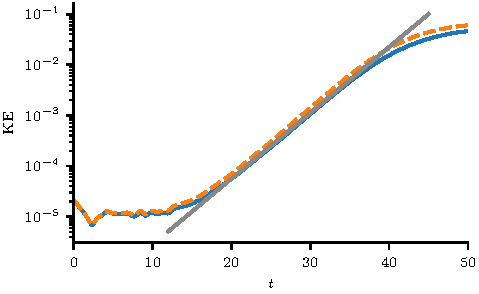
\includegraphics[width=0.5\linewidth]{log_kinetic_energy_over_time.pdf}
  \caption{\textit{Logarithmic plot of the total kinetic
      energy during the linear phase.} Overlaid is a straight
    line corresponding to the linear growth rate $\sigma = 0.13$. The
    isotropic case is represented as a blue, solid line and the
    switching case as an orange, dashed line. Though the kinetic energy is initially slightly greater using the switching model, the growth rate appears unaffected by choice of viscosity model. The duration of the linear phase also appears to be negligibly affected.}%
  \label{fig:log_kinetic_energy_over_time}
\end{figure}

The linear development of the kink instability lasts until $t\approx 35$ as illustrated in   Figure~\ref{fig:log_kinetic_energy_over_time} and has a measured linear growth rate of $\sigma = 0.13$. Since the initial velocity perturbation is calculated from an ideal and inviscid MHD model with a piecewise constant $\alpha(r)$ in the equilibrium configuration, the perturbation does not necessarily represent the most unstable mode for the setup of the simulation. For this reason there is a brief transient period before the exponential rise of the instability at $t\approx10$, as shown in Figure~\ref{fig:log_kinetic_energy_over_time}. The isotropic model damps this initial velocity perturbation more than the switching model, leading to a small difference in kinetic energy during the growth of the linear instability, although the growth rate appears to be identical across the two models. The duration of the linear phase is also unaffected by the choice of viscosity model.

\begin{figure}[t]
  \centering
    \begin{subfigure}{0.49\textwidth}
      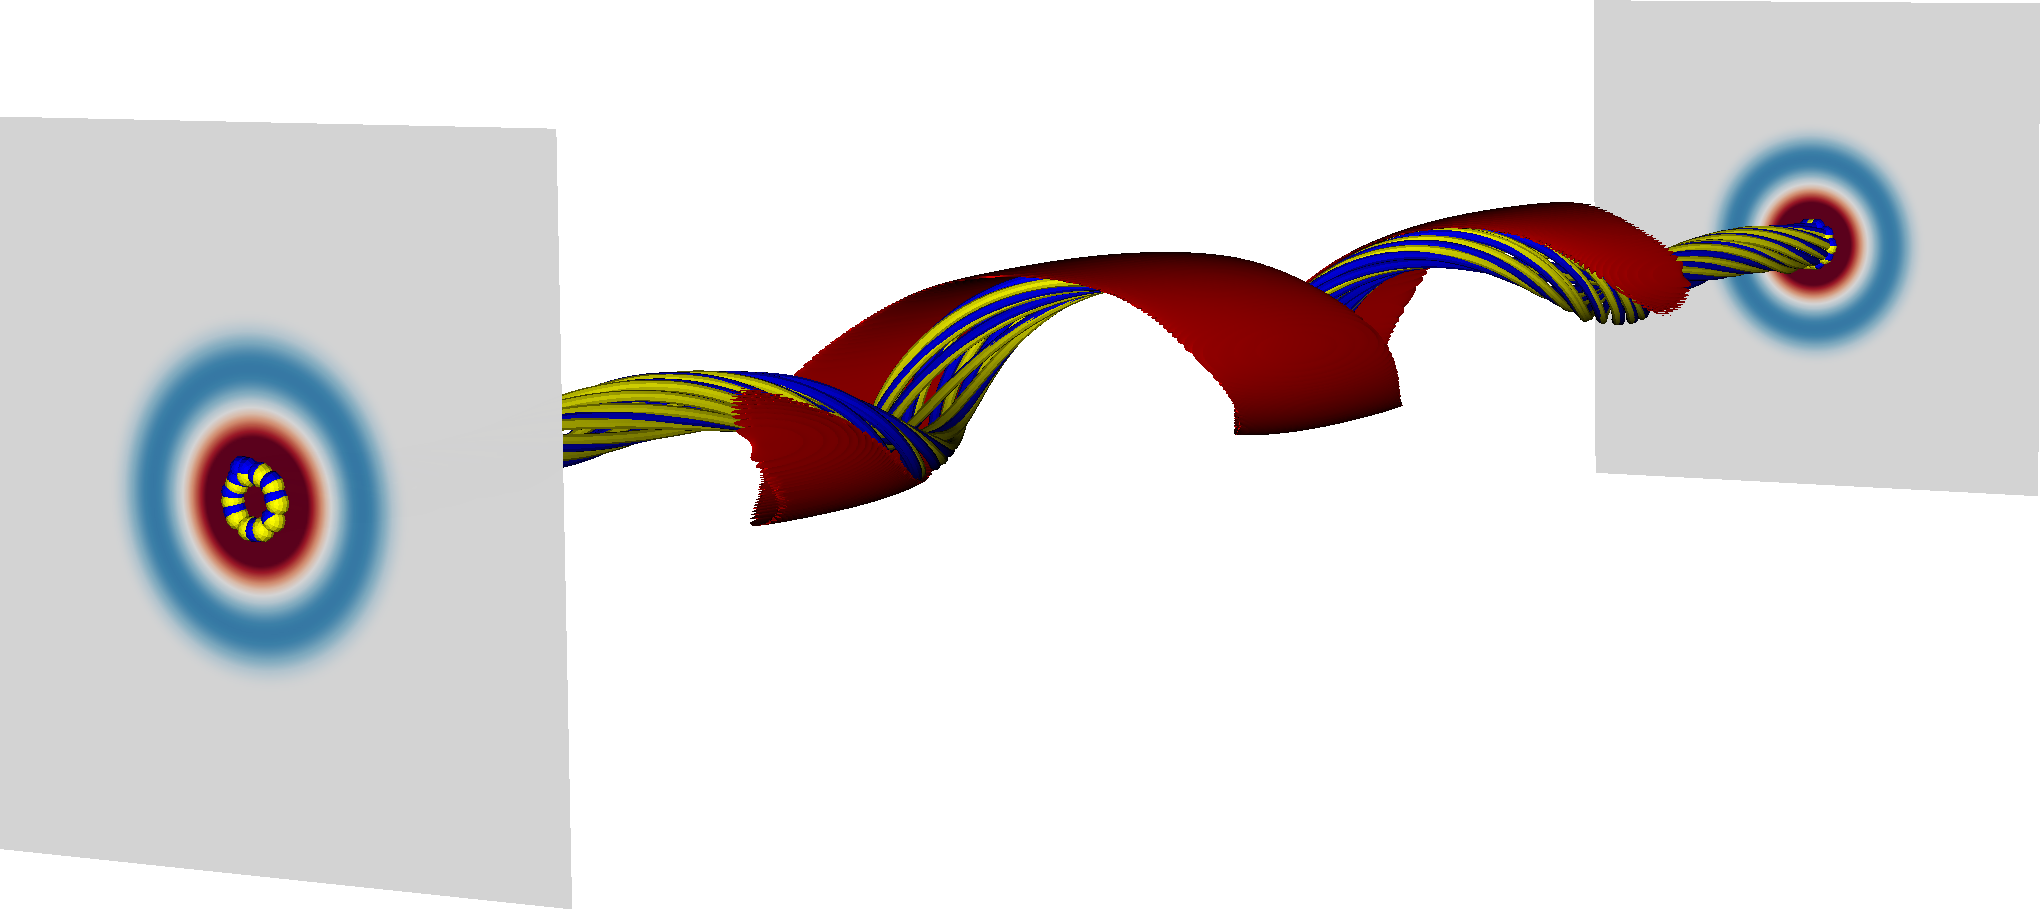
\includegraphics[width=\linewidth]{field_line_plots/cropped/v1e-4r5e-4.5-isotropic_0009_cropped.png}
      \caption{$t=45$}
      \label{fig:field_lines_0009}
    \end{subfigure}
    \begin{subfigure}{0.49\textwidth}
      \includegraphics[width=\linewidth]{field_line_plots/cropped/v1e-4r5e-4.5-isotropic_0010_cropped.png}
      \caption{$t=50$}
      \label{fig:field_lines_0010}
    \end{subfigure}
\caption{\textit{The transition from linear to nonlinear instability in the isotropic case.} The yellow field lines start at $z=10$ and the blue field lines at $z=-10$. The isosurfaces are at $|\vec{\jmath}| = 4$. The slices are plots of $\alpha(r)$. The linear growth of the instability ends around $t=35$ and the inner field compresses into the outer field, creating a current sheet. Between $t=45$ and $50$ this current sheet enables reconnection between the two regions. The transition for the switching case is qualitatively similar. In all three plots, $\nu = 10^{-4}$ and $\eta = 5\times 10^{-4.5}$, respectively.}
\label{fig:reconnecting_field_lines}%
\end{figure}

Initially, the instability occurs in the inner region of twist, $r<0.5$, where the magnetic field kinks helically. This section of the magnetic field compresses into the outer region, creating a current sheet along the length of the tube as shown in Figure~\ref{fig:field_lines_0009}. As the field continues to be compressed, it provides a magnetic pressure force that stalls the linear growth. The greater kinetic energy in the switching case leads to greater compression and thus a larger (though not notably stronger) current sheet. After this point, the growth of the kink instability is no longer in the linear phase.

During the transition from the linear to the nonlinear phase, field lines in the current sheet between the regions of inner and outer twist start to reconnect (Figures~\ref{fig:reconnection-field-lines}). This happens sooner in the switching case, due to the larger compression.

\subsection{Nonlinear phase}

\begin{figure}[t]
    \centering
    \begin{subfigure}[t]{0.49\textwidth}
      \centering
      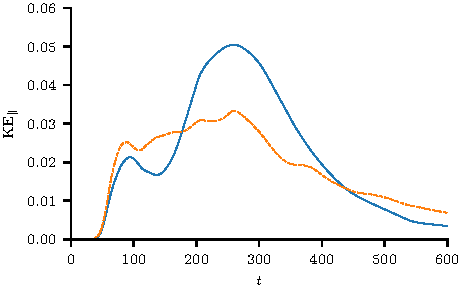
\includegraphics[width=\linewidth]{parallel_kinetic_energy_over_time.pdf}
      \caption{Parallel kinetic energy}
      \label{fig:parallel_kinetic_energy_over_time}
    \end{subfigure}%
    \begin{subfigure}[t]{0.49\textwidth}
      \centering
      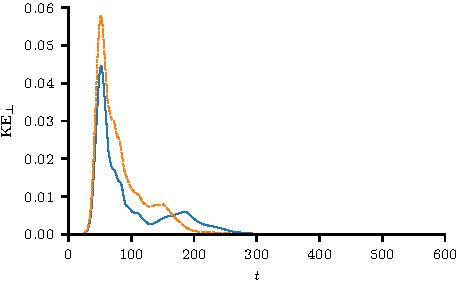
\includegraphics[width=\linewidth]{perp_kinetic_energy_over_time.pdf}
      \caption{Perpendicular kinetic energy}
      \label{fig:perp_kinetic_energy_over_time}
    \end{subfigure}
    \begin{subfigure}[t]{0.49\textwidth}
      \centering
      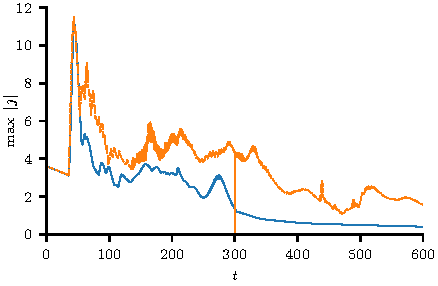
\includegraphics[width=\linewidth]{current_density_over_time.pdf}
      \caption{Maximum current density}
      \label{fig:current_density_over_time}
    \end{subfigure}
    \begin{subfigure}[t]{0.49\textwidth}
      \centering
      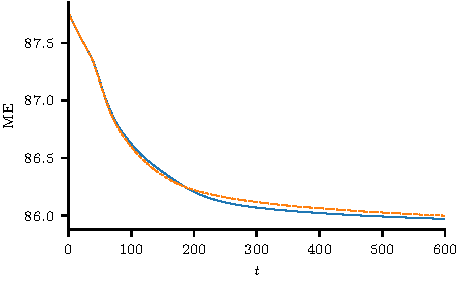
\includegraphics[width=\linewidth]{magnetic_energy_density_over_time.pdf}
      \caption{Magnetic energy}
      \label{fig:magnetic_energy_density_over_time}
    \end{subfigure}
    \caption{\textit{Energy components and current as functions of time.} Both isotropic (blue, solid) and switching (orange, dashed) viscosity models are shown, with diffusion parameters $\nu = 10^{-4}$ and $\eta = 5\times 10^{-4.5}$.}
    \label{fig:energies}
\end{figure}

Although the choice of viscosity model has a small effect on the
linear phase of the kink instability, it does play an important role
in the development of the nonlinear phase. By examining the kinetic
energies (KEs) in Figures~\ref{fig:energies}(a) and (b), a pattern
emerges in both cases that has similarities with the nonlinear
  behaviour of kink instabilities described in Hood et
al.~\cite{hoodCoronalHeatingMagnetic2009}. Shortly after the linear
phase, at $t\approx50$, the KEs for both viscosity models
exhibits a sharp rise, with the KEs associated with the switching
model attaining higher amplitudes. At the same time, a sharp rise is
also found in the maximum current as seen in
Figure~\ref{fig:energies}(c) and, leading on from this spike, the
current magnitudes associated with the switching model are larger than
those associated with the isotropic model. Returning to the KEs, the
energies associated with the switching model are greater until
$t\approx175$, after which, in \emph{only} the isotropic case, 
a clear secondary spike in perpendicular kinetic energy is found, along with a large
increase in parallel kinetic energy, much greater than the corresponding energy
found in the switching case. It is difficult to detect this new phase
in the maximum current (Figure~\ref{fig:energies}(c)), but it is found
in other quantities related to magnetic reconnection. 

\begin{figure}[t]
    \centering
    \begin{subfigure}[t]{0.5\textwidth}
      \centering
      \includegraphics[width=\linewidth]{max_parallel_electric_field.pdf}
      \caption{Parallel electric field}
      \label{fig:max_parallel_electric_field}
    \end{subfigure}%
    ~
    \begin{subfigure}[t]{0.5\textwidth}
      \centering
      \includegraphics[width=\linewidth]{mean_difference_in_connectivity.pdf}
      \caption{Difference in connectivity}
      \label{fig:mean_difference_in_connectivity}
    \end{subfigure}
    \caption{\textit{Reconnection rates.} The maximum integrated parallel electric field and mean difference in connectivity are plotting for the isotropic (blue dot \& solid line) and switching (orange cross \& dashed line) cases with $\nu = 10^{-4}$ and $\eta = 5\times 10^{-4.5}$. The difference in time between each data point is $5$ Alfv\'en times.}
    \label{fig:reconnection-rates}
\end{figure}

Figure~\ref{fig:reconnection-rates} displays the time series of the maximum integrated parallel electric field and the mean difference in connectivity, for both viscosity models. Both of the time series in Figure~\ref{fig:reconnection-rates} display similar trends to those found in the perpendicular kinetic energy plot, Figure~\ref{fig:energies}(a). For both isotropic and anisotropic viscosity there appears to be two major peaks in the reconnection measures that align with peaks in the perpendicular kinetic energy. This is much more obvious in the isotropic case. Both viscosity models allow for two phases of reconnection but the time at which they occur is significantly modified by the form of viscosity chosen. It is, therefore, clear that the form of viscosity is having a significant effect on the nonlinear evolution of the kink instability, both on the flow dynamics and the reconnection of the magnetic field. The following section presents, in more detail, the two important phases indicated by the isotropic time series, and how the results differ in the switching case.

\subsection{First phase: $t\approx65$--$100$}

\begin{figure}[t]
  \centering
  \begin{subfigure}[t]{0.32\textwidth}
    \centering
    \includegraphics[width=\linewidth]{slices/final_isotropic_current_density_0013.pdf}
    \caption{iso; $t=65$}
    \label{fig:final_isotropic_current_density_0013}
  \end{subfigure}
  \hfill
  \begin{subfigure}[t]{0.32\textwidth}
    \centering
    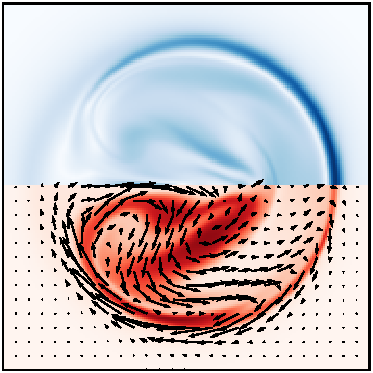
\includegraphics[width=\linewidth]{slices/final_isotropic_current_density_0015.pdf}
    \caption{iso; $t=75$}
    \label{fig:final_isotropic_current_density_0015}
  \end{subfigure}
  \hfill
  \begin{subfigure}[t]{0.32\textwidth}
    \centering
    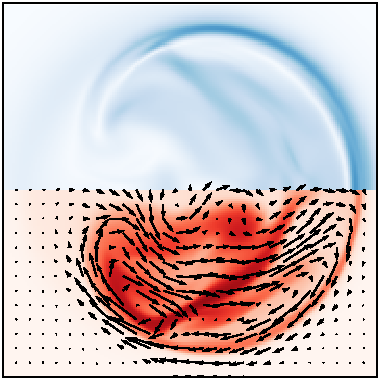
\includegraphics[width=\linewidth]{slices/final_isotropic_current_density_0020.pdf}
    \caption{iso; $t=100$}
    \label{fig:final_isotropic_current_density_0020}
  \end{subfigure}
  \hfill
  \begin{subfigure}[t]{0.32\textwidth}
    \centering
    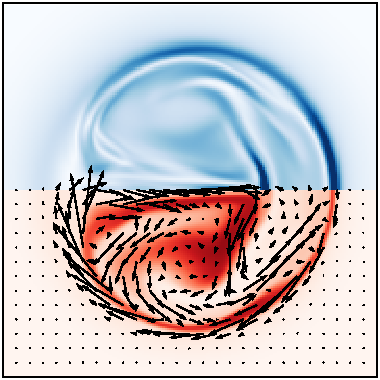
\includegraphics[width=\linewidth]{slices/final_switching_current_density_0013.pdf}
    \caption{swi; $t=65$}
    \label{fig:final_switching_current_density_0013}
  \end{subfigure}
  \hfill
  \begin{subfigure}[t]{0.32\textwidth}
    \centering
    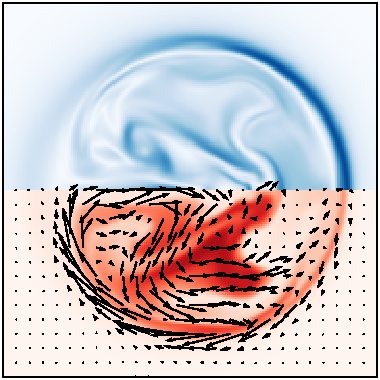
\includegraphics[width=\linewidth]{slices/final_switching_current_density_0015.pdf}
    \caption{swi; $t=75$}
    \label{fig:final_switching_current_density_0015}
  \end{subfigure}
  \hfill
  \begin{subfigure}[t]{0.32\textwidth}
    \centering
    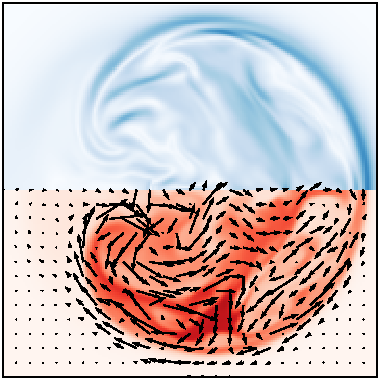
\includegraphics[width=\linewidth]{slices/final_switching_current_density_0020.pdf}
    \caption{swi; $t=100$}
    \label{fig:final_switching_current_density_0020}
  \end{subfigure}
  \caption{\textit{The difference in the evolution of current density,
      temperature and velocity structures between the isotropic
        and the switching viscosity cases}. Slices at $z=0$ of
    current density (top of each figure; blue is $|\vec{\jmath}| =
    3.5$, white is $|\vec{\jmath}| = 0$) and temperature (bottom of
    each figure; red is $T = 5\times10^{-2}$, white is
    $T=1.15\times10^{-5}$), overlaid with fluid flow. The halves shown are identical to their unseen counterparts, for both temperature and current density. That is, the simulation is vertically symmetrical at these times. The profile is cropped to
    $x=\pm1,\ y=\pm1$. The top three panels show the
    isotropic case and the bottom three panels show the switching case.}
  \label{fig:turning-point}
\end{figure}

At $t=65$, an intense current structure appears near the centre of the
tube for both viscosity models, although it is much stronger in the
switching case as illustrated in Figure~\ref{fig:turning-point}. Since the viscous damping associated with parallel viscosity is much less than that of isotropic viscosity, the flows in the switching case are stronger than those in the isotropic case (Figures~\ref{fig:energies}(a) and (b)). The faster flows drive stronger reconnection in the central current structure (see Figure~\ref{fig:reconnection-rates}) and the interaction of these processes leads to stronger outflows and finer-scale structures in the switching model case compared with the isotropic model case. Evidence of this behaviour can be seen by comparing the current and flow structures in Figure~\ref{fig:turning-point}. The effects of this phase can also be seen in the magnetic energy evolution, shown in Figure~\ref{fig:energies}(d). Between times $t=100$ and $125$, due to stronger reconnection in the switching case, the magnetic field relaxes marginally faster than that of the isotropic case, before the secondary instability begins in the isotropic case around $t=125$.

\begin{figure}[t]
  \centering
  \begin{subfigure}[t]{0.32\textwidth}
    \centering
    \includegraphics[width=\linewidth]{slices/final_isotropic_current_density_0025.pdf}
    \caption{iso; $t=125$}
    \label{fig:final_isotropic_current_density_0025}
  \end{subfigure}
  \hfill
  \begin{subfigure}[t]{0.32\textwidth}
    \centering
    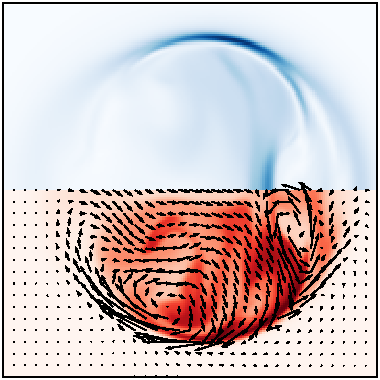
\includegraphics[width=\linewidth]{slices/final_isotropic_current_density_0030.pdf}
    \caption{iso; $t=150$}
    \label{fig:final_isotropic_current_density_0030}
  \end{subfigure}
  \hfill
  \begin{subfigure}[t]{0.32\textwidth}
    \centering
    \includegraphics[width=\linewidth]{slices/final_isotropic_current_density_0035.pdf}
    \caption{iso; $t=175$}
    \label{fig:final_isotropic_current_density_0035}
  \end{subfigure}
  \hfill
  \begin{subfigure}[t]{0.32\textwidth}
    \centering
    \includegraphics[width=\linewidth]{slices/final_switching_current_density_0025.pdf}
    \caption{swi; $t=125$}
    \label{fig:final_switching_current_density_0025}
  \end{subfigure}
  \hfill
  \begin{subfigure}[t]{0.32\textwidth}
    \centering
    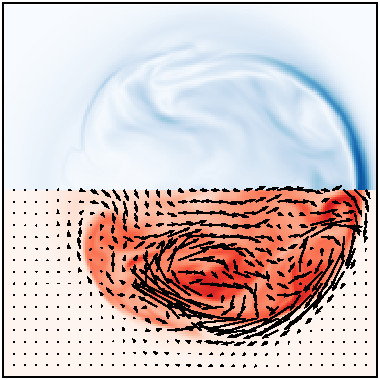
\includegraphics[width=\linewidth]{slices/final_switching_current_density_0030.pdf}
    \caption{swi; $t=150$}
    \label{fig:final_switching_current_density_0030}
  \end{subfigure}
  \hfill
  \begin{subfigure}[t]{0.32\textwidth}
    \centering
    \includegraphics[width=\linewidth]{slices/final_switching_current_density_0035.pdf}
    \caption{swi; $t=175$}
    \label{fig:final_switching_current_density_0035}
  \end{subfigure}
  \caption{\textit{The formation of a reconnection feedback loop in the isotropic and the switching viscosity cases.} Plotting parameters are identical to those of Figure~\ref{fig:turning-point}. The isotropic case shows two current sheets causing reconnection at the top and bottom of the tube, producing flows that sustains another central current sheet, which feeds back into the top and bottom sheets. The switching case instead shows one single main current sheet at the right hand side, along with numerous smaller current structures throughout the domain.}
  \label{fig:feedback-reconnection}
\end{figure}

\subsection{Second phase: $t\approx125$--$175$}
The contrast between fine-scale current and flow structures for the switching model, and the smoother, larger-scale structures of the isotropic model continues to be present at later times. Figure~\ref{fig:feedback-reconnection} shows the same data as Figure~\ref{fig:turning-point} but for the times $t=125$, $150$ and $175$. Looking at the slices for $t=125$, there is more fine-scale structure generated in the switching case compared to the isotropic case, as in the first phase described above. This second phase, however, marks the beginning of a significant change in behaviour in the isotropic model case. From Figure~\ref{fig:energies}, the parallel KE for the isotropic model exhibits a rapid and large increase in kinetic energy, characteristic of a secondary instability. To a lesser extent, there is also growth in the perpendicular KE, and the two reconnection measures for the isotropic model. In the second phase, these three measures increase to eventually become greater than their corresponding values for the switching model, around $t=175$. The significant difference in the behaviour between the two models are explored by first considering the slices in Figure~\ref{fig:feedback-reconnection}.

\begin{figure}[t]
  \centering
  \begin{subfigure}[b]{0.48\textwidth}
    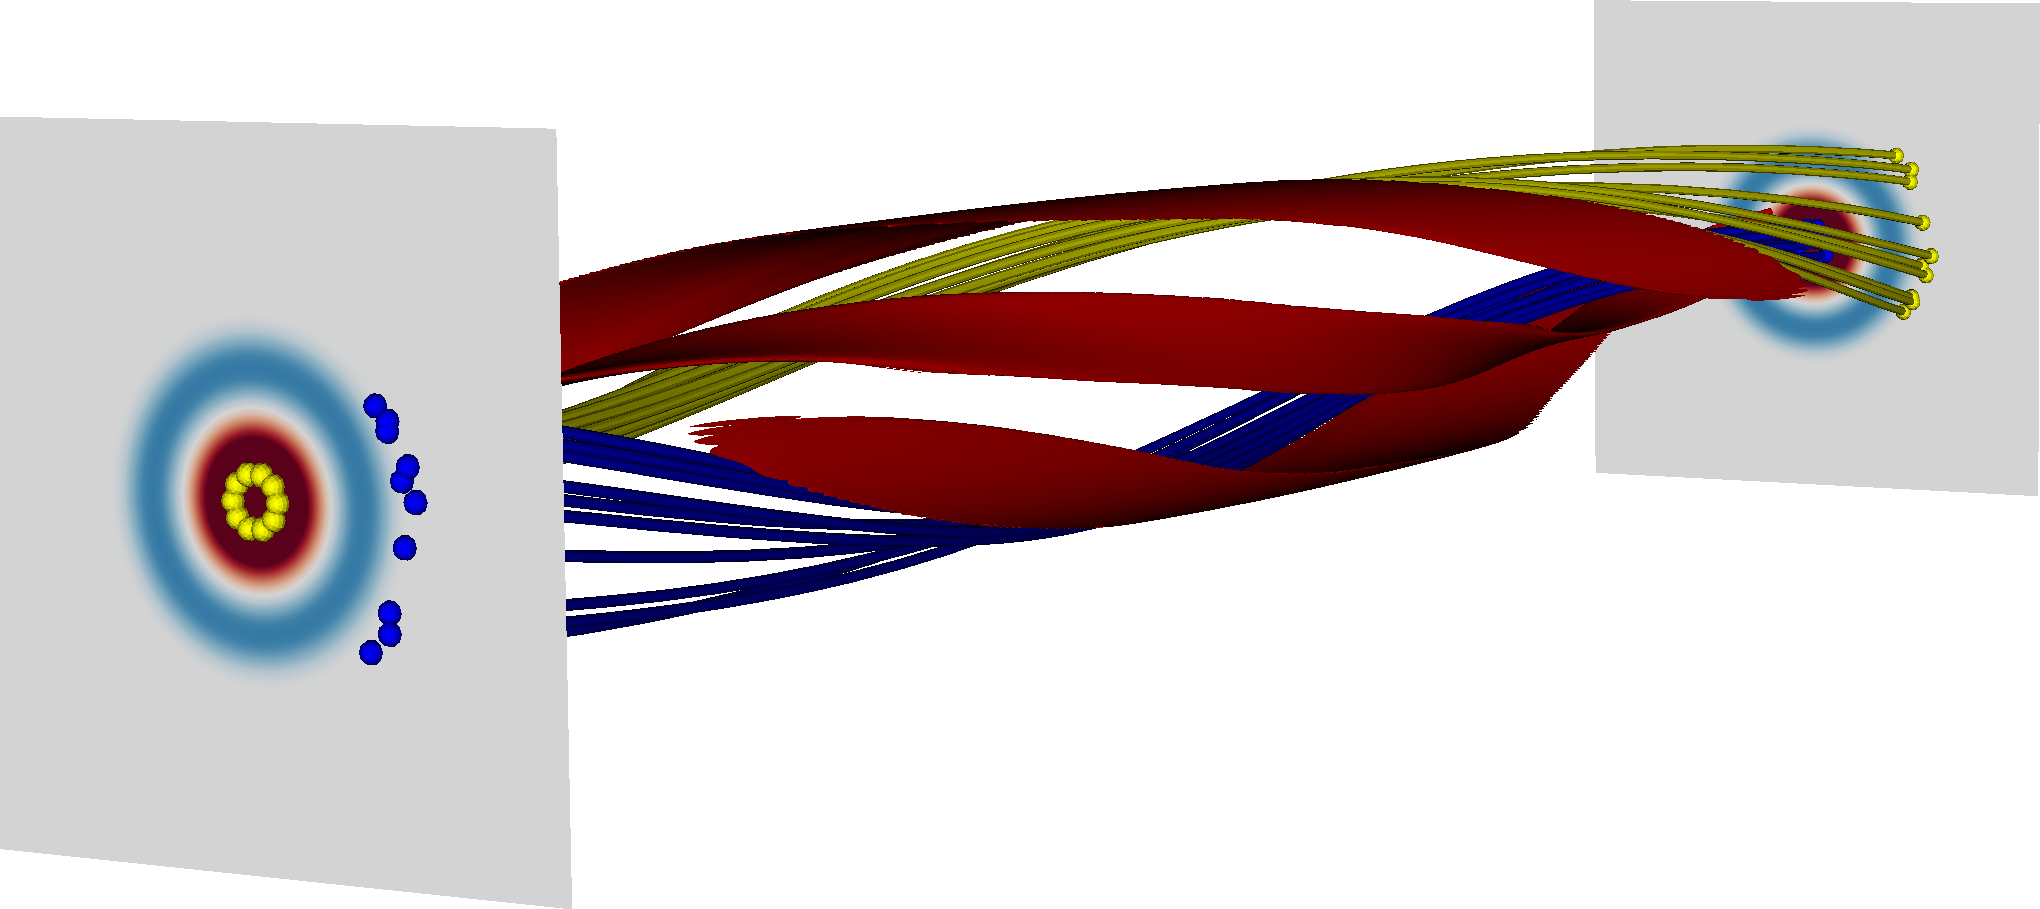
\includegraphics[width=\linewidth]{field_line_plots/cropped/v1e-4r5e-4.5-isotropic_0035_cropped.png}
    \caption{Isotropic}
    \label{fig:reconnection-field-lines-iso}
  \end{subfigure}
  \begin{subfigure}[b]{0.48\textwidth}
    \includegraphics[width=\linewidth]{field_line_plots/cropped/v1e-4r5e-4.5-switching_0035_cropped.png}
    \caption{Switching}
    \label{fig:reconnection-field-lines-swi}
  \end{subfigure}
  \caption{\textit{The difference in 3D current structures at $t=175$.} Isosurfaces are at $|\vec{\jmath}| = 1.5$.}
\label{fig:reconnection-field-lines}
\end{figure}

At $t=125$ (panels (a) and (d) of Figure~\ref{fig:feedback-reconnection}), the difference in behaviour
between the models is similar to the first phase but some new features
appear. The KE in the isotropic model begins to increase and, as
mentioned before, appears to signify a secondary instability. In
Figure~\ref{fig:feedback-reconnection}(a), two new current sheets have
formed at the top and bottom of the tube. A three-dimensional (3D)
visualisation of these current sheets is shown in
Figure~\ref{fig:reconnection-field-lines-iso}. The outflow from the
reconnection occurring within these current sheets then creates two
new symmetric vortices on the right hand side of the tube, advecting
the field into the centre of the tube. This behaviour can be seen
clearly in Figure~\ref{fig:feedback-reconnection}(b) where vortex
motion compresses the magnetic field and forms a central region of
enhanced current density. Later, as seen at $t=175$ in Figure~\ref{fig:feedback-reconnection}(c), the central current region becomes stronger due to continued compression and reconnection ensues, becoming stronger than the switching model case (see Figure~\ref{fig:reconnection-rates}). The outflows from this current region then feed into the vortical motions that drive the compression. In this way, a feedback loop is set up, and the reconnection within the current structure continuously drives the flow, resulting in an instability. This kind of interaction between multiple current sheets is also seen in~\cite{hoodCoronalHeatingMagnetic2009}. Due to this secondary instability, magnetic relaxation now becomes faster for the isotropic case. The magnetic energy for this case now dips below that of the switching case, as shown in Figure~\ref{fig:energies}(d).

During this phase, the kinetic energy in the switching model case also increases but to a much smaller extent compared to the isotropic model case. Although the current densities in Figures~\ref{fig:feedback-reconnection}(d) to (f) again exhibit finer-scale structure compared to the isotropic case, the magnitude of the current density within the tube becomes weaker with a more uniform profile developing in time. The dominating current sheets are on the edge of the tube, as also indicated in Figure~\ref{fig:reconnection-field-lines-swi}.

\subsection{Late-time states}

\begin{figure}[t]
  \centering
  \begin{subfigure}[b]{0.48\textwidth}
    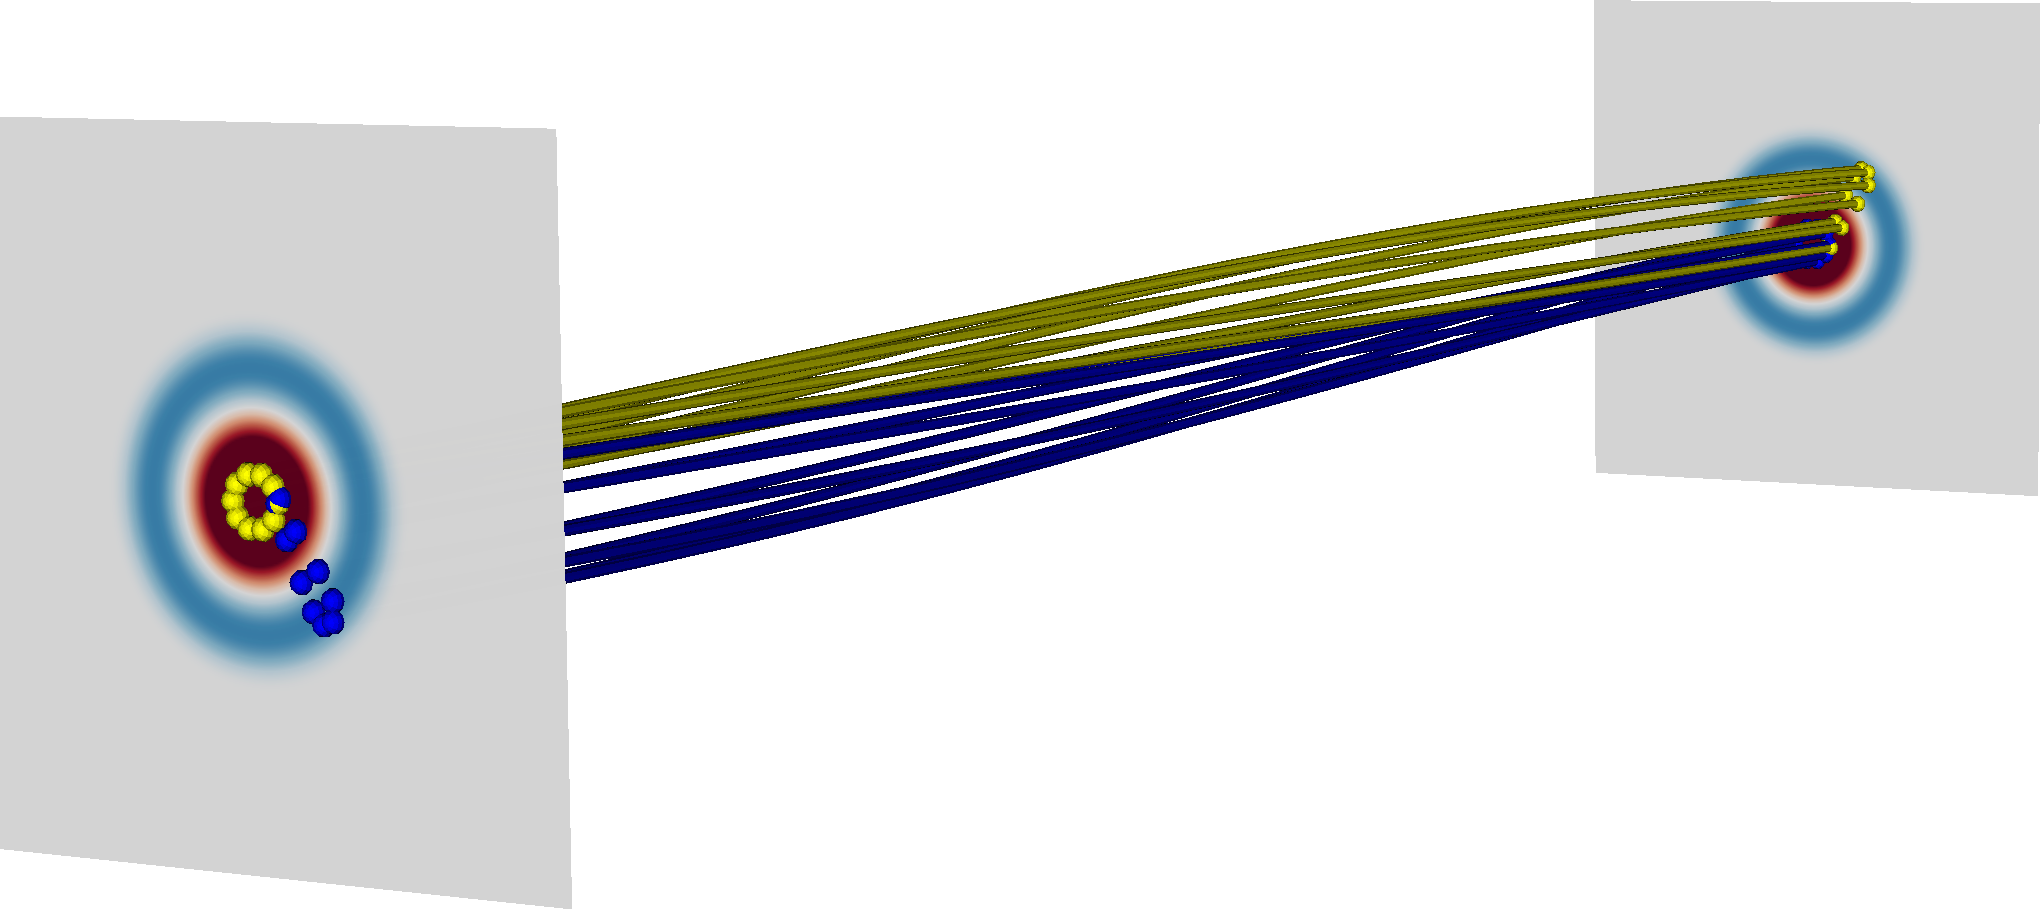
\includegraphics[width=\linewidth]{field_line_plots/cropped/v1e-4r5e-4.5-isotropic_0062_cropped.png}
    \caption{Isotropic}
  \end{subfigure}
  \begin{subfigure}[b]{0.48\textwidth}
    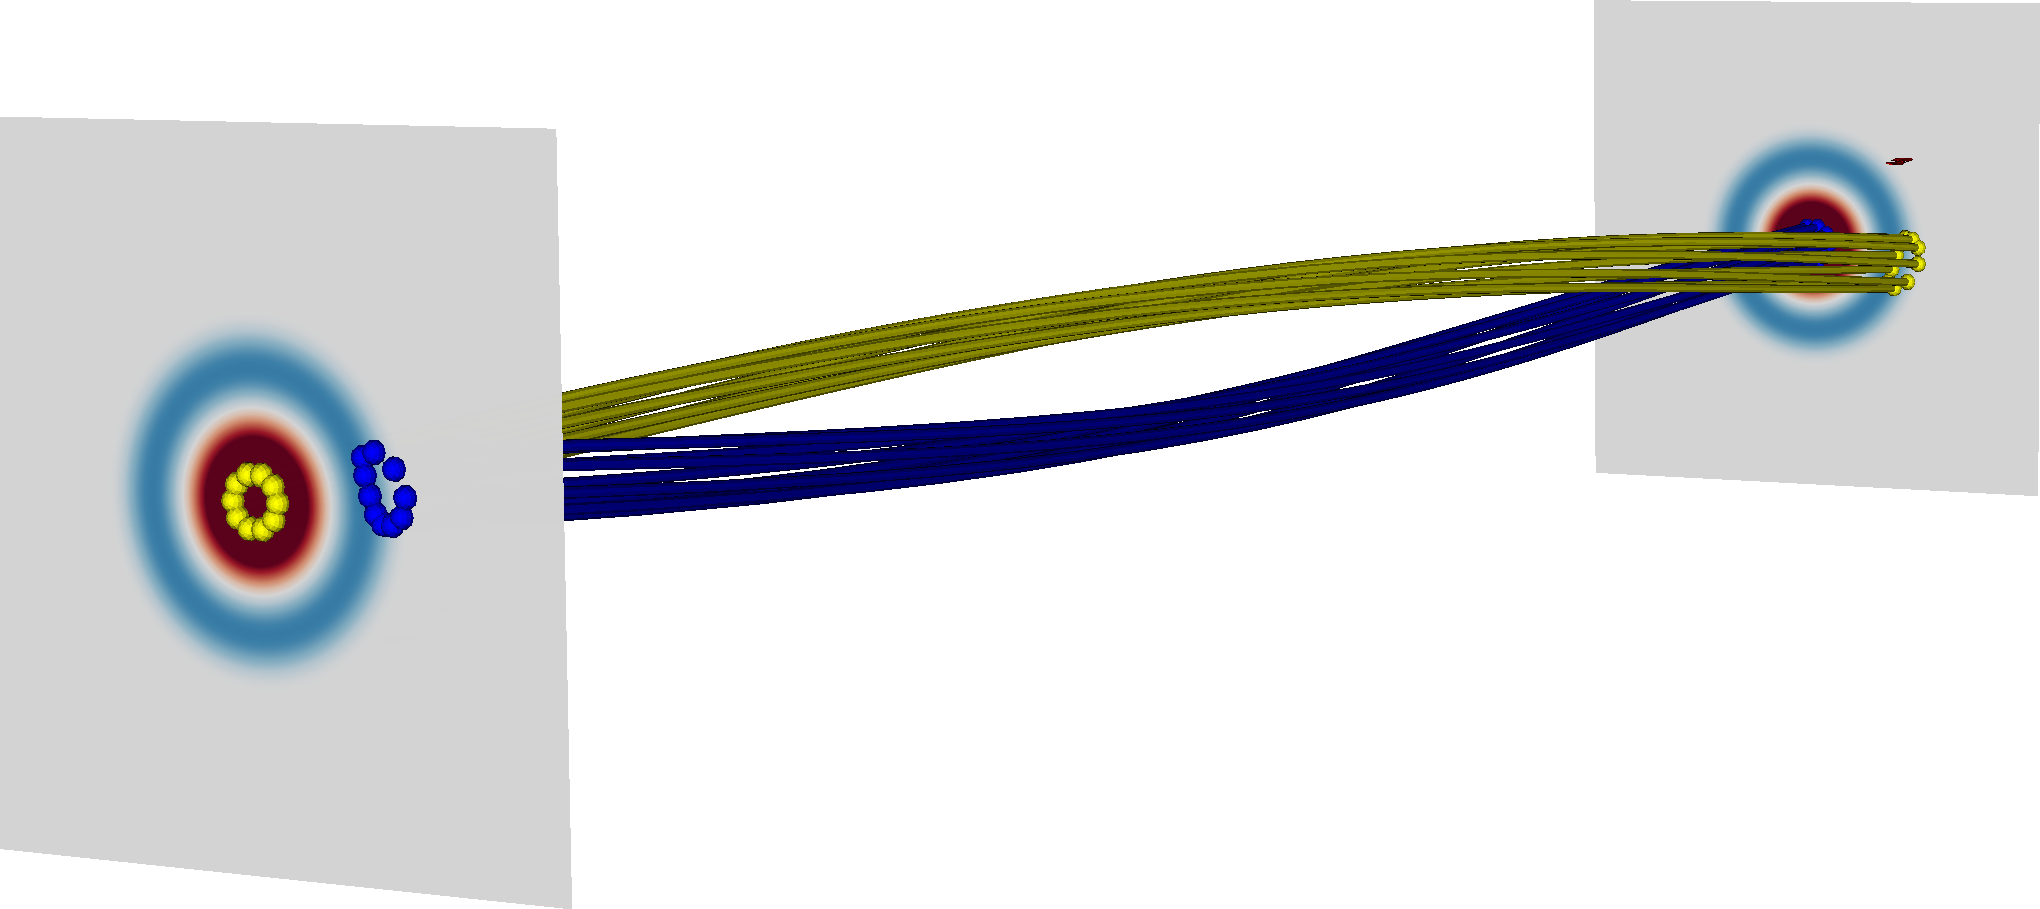
\includegraphics[width=\linewidth]{field_line_plots/cropped/v1e-4r5e-4.5-switching_0059_cropped.png}
    \caption{Switching}
  \end{subfigure}
  \caption{\textit{Late-time magnetic field structures at $t=600$.}}
\label{fig:finale-field-lines}
\end{figure}

For both cases, the asymptotic relaxed magnetic field is a linear force-free field. The route to this asymptotic state, however, depends on the viscosity model used. At the late time of $t=600$, there remain clear differences in the field structure between the two models resulting from the different nonlinear evolutions, as can be seen in Figure~\ref{fig:finale-field-lines}. At $t=600$, the magnetic field in the isotropic case (Figure~\ref{fig:finale-field-lines}(a)) appears straighter, indicative of more efficient magnetic relaxation. Indeed, Figure~\ref{fig:energies}(d) shows that more energy has been extracted from the field in the isotropic case. At $t=600$, the current density and energies (see Figure~\ref{fig:energies}) are still non-zero, so further relaxation is expected. For coronal applications, however, these late times are not as important as the early phases, described above, when the initial and secondary instabilities develop.

\subsection{Viscous and Ohmic heating}

\begin{figure}[t]
    \centering
    \begin{subfigure}[t]{0.32\textwidth}
      \includegraphics[width=\textwidth]{ohmic_heating_over_time.pdf}
      \caption{Ohmic heating}
    \end{subfigure}
    \begin{subfigure}[t]{0.32\textwidth}
      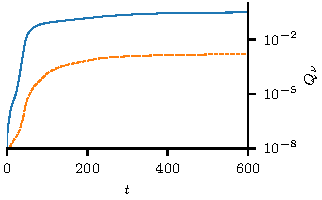
\includegraphics[width=\textwidth]{viscous_heating_over_time.pdf}
      \caption{Viscous heating}
    \end{subfigure}
    \begin{subfigure}[t]{0.32\textwidth}
      \includegraphics[width=\textwidth]{total_heating_over_time.pdf}
      \caption{Total heating}
    \end{subfigure}
    \caption{\textit{Heating rates as functions of time.} Plots are shown for isotropic (blue, solid) and switching (orange, dashed) viscosity, with diffusion parameters $\nu = 10^{-4}$ and $\eta = 5\times 10^{-4.5}$. Ohmic heating dominates isotropic viscous heating by an order of magnitude, and switching viscosity by four orders. Isotropic viscosity generates a factor of around $10^{3}$ more heat that switching viscosity. Even though more Ohmic heat is generated in the switching case, it does not compensate for the much weaker viscous heating.}
    \label{fig:heating}
\end{figure}

Over the lifetime of the entire instability the switching model allows for the generation of more Ohmic heating (Figure~\ref{fig:heating}(a)). This is despite the long, secondary phase of reconnection produced in the isotropic case. The greater heating in the switching case is due to two factors: the greater compression created by faster flows, creating stronger or larger current sheets and the more numerous current sheets created by more complex flows. However, isotropic viscous heating dominates that of the switching model by two orders of magnitude (Figure~\ref{fig:heating}(b)) ultimately leading to greater overall heating in the isotropic case (Figure~\ref{fig:heating}(c)). Physically, this is due to anisotropic viscosity only performing significant damping when velocity gradients align appropriately with the magnetic field (that is, when $(\ten{W} \vec{b}) \cdot \vec{b}$ is non-zero). 

Comparing Ohmic and viscous heating (Figures~\ref{fig:heating}(a) and (b)), Ohmic heating outperforms viscous heating in both cases, by an order of magnitude in the isotropic case and by three orders in the switching case. Even though similar values for the diffusion of the magnetic field $\eta$ and the velocity $\nu$ are used, during the kink instability the current sheets produced are much stronger than the gradients in velocity, hence the Ohmic heating dissipates more energy than the viscous heating.

Due to the relationship between $(\ten{W} \vec{b}) \cdot \vec{b}$ and $Q_{\nu}$ (equation~\eqref{eq:aniso_viscous_heating} with $s\approx 1$), the small magnitude of $Q_{\nu}$ in Figure~\ref{fig:heating}(b) implies that $(\ten{W} \vec{b}) \cdot \vec{b}$ is small everywhere. With the anisotropic viscous heating being heavily dependent on the magnetic field direction and since $(\ten{W} \vec{b}) \cdot \vec{b}$ is small everywhere in the kink simulation, it follows that the anisotropic viscous heating is always lower in magnitude compared to the isotropic viscous heating, which is not bound by the diection of the magnetic field.

\subsection{The effect of anisotropy on feedback reconnection}

I have described the nonlinear evolution of the kink instability for the cases of only isotropic viscosity and only anisotropic viscosity. When the viscosity is totally isotropic, the secondary instability is found, yet when the viscosity is totally anisotropic, the same instability is disrupted. To determine how anisotropic the viscosity must become before the secondary instability is disrupted, the degree of anisotropy can be fixed by artificially fixing the value of $s$ to some constant, instead of letting $s$ rely on the local field strength $|\vec{B}|$. It should be noted that the simulations in which $s$ is fixed are no longer physically realistic, but the results can be used to estimate the degree of anisotropy required in the viscosity to disrupt the secondary instability. Since the interpolation involves only $s^2$ instead of $s$, in practice the value of $s^2$ is fixed.

\begin{figure}[t]
  \centering
  \includegraphics[width=0.5\linewidth]{kinetic-energy-changing-s.pdf}
  \caption{\textit{Kinetic energy over time, varying the switching
        function $s^2$.} The grey lines are the two regular cases; switching, where $s^2 = 1$ (dashed), and isotropic (solid), where $s^2=0$. The coloured lines represent values of $s^2 = 0.5$ (blue, dotted), and $s^2 = 0.6$ (orange, dash-dotted). There is a clear critical value somewhere between $0.5$ and $0.6$, where the behaviour changes.}
  \label{fig:kinetic-energy-changing-s}
\end{figure}

By letting $s^2$ in equation~\eqref{eq:switching_model} take values between $0$ and $1$, it is found that there is not a smooth transition between the two extremes of behaviour. Instead, there is a critical value of $s^2$, between $0.5$ and $0.6$, below which (closer to isotropic) the resultant flows are simple enough to create and sustain feedback reconnection, and above which (closer to anisotropic) the flows are sufficiently complex to disrupt the secondary instability. This behaviour can be seen in how the kinetic energy time series changes with $s^2$ in Figure~\ref{fig:kinetic-energy-changing-s}.

\section{Parameter study}
\label{sec:results2}

In order to confirm that the results of Section~\ref{sec:results} are typical, and to further understand how they vary, two parameter studies are performed; one varying viscosity, keeping all other parameters constant; and one varying resistivity, again keeping all other parameters constant. 

In the first study the viscosity is varied as $\nu = 5 \times 10^{-n}$, where the index $n$ takes the values $4.75$, $4.5$, $4.25$, $4$ and $3.75$, while keeping resistivity constant at $\eta = 5\times10^{-4.5}$. This range of viscosities represents values that are typically used in simulations, with a lower bound above numerical diffusion and an upper bound below physically unrealistic values for the corona.

In the second study the resistivity is similarly varied as $\eta = 5 \times 10^{-m}$, where the index $m$ takes the values $4.75$, $4.5$, $4.25$, $4$, $3.75$, and $3.5$, while keeping the resistivity constant at $\nu = 5\times 10^{-4.5}$. Similar to the limits on viscosity, any lower resistivities become comparable to numerical diffusion. Higher resistivities diffuse the field so quickly that the instability does not have time to grow.

\subsection{Effect on the secondary instability varying diffusion parameters}
\label{sec:secondary_instability}

\begin{figure}[t]
    \centering
    \begin{subfigure}[t]{0.5\textwidth}
      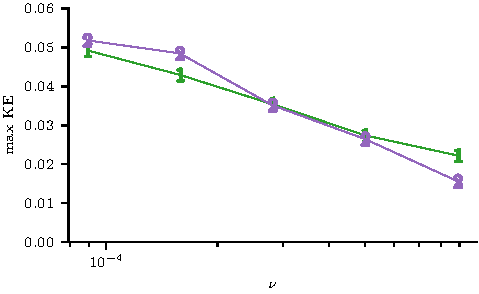
\includegraphics[width=\textwidth]{max_ke_split_inst_changing_viscosity.pdf}
      \caption{Varying viscosity; $\eta = 5\time 10^{-4.5}$}
    \end{subfigure}%
    ~
    \begin{subfigure}[t]{0.5\textwidth}
      \includegraphics[width=\textwidth]{max_ke_split_inst_changing_resistivity.pdf}
      \caption{Varying resistivity; $\nu = 5\time 10^{-4.5}$}
    \end{subfigure}
    \caption{\textit{Maximum kinetic energy corresponding to initial instability and secondary instability as functions of resistivity $\eta$ and viscosity $\nu$.} In both plots are shown the maximum kinetic energy produced by the initial instability (green, $1$-marker) and the maximum kinetic energy produced by the secondary instability (purple, $2$-marker). Only results using the isotropic viscosity are shown.}
    \label{fig:secondary_instability}
\end{figure}

Figure~\ref{fig:secondary_instability} shows the maximum kinetic energy produced by the two instabilities found in the isotropic case in Section~\ref{sec:results}. The maximum kinetic energy provides a useful measure of the efficacy of an instability, particularly when comparing the relative magnitudes of the initial and secondary instabilities. Since only the isotropic case reveals evidence of the secondary instability, results from the switching case are not shown.

Looking at Figure~\ref{fig:secondary_instability}(a), it is observed that increasing $\nu$ reduces the kinetic energy generated in both instabilities. For small values of $\nu$ the secondary instability causes more energy to be produced than the first, however as $\nu$ increases, this relationship reverses, with the initial instability causing more energy to be produced than the secondary one for large $\nu$. This reversal suggests that the greater kinetic energy produced by the initial instability for low values of $\nu$ is causing a stronger current sheet to form, enhancing reconnection, and producing a stronger secondary instability.

The effect of resistivity $\eta$ on the secondary instability is to suppress it entirely when $\eta$ is large. Since the secondary instability is driven by reconnection outflows, it is not surprising that there are values of $\eta$ for which the reconnection outflows do not feedback to produce the instability.

\subsection{Varying viscosity}

\label{sec:visc_param_study}

\subsubsection{Dependence of heating on viscosity}

\begin{figure}[t]
    \centering
    \begin{subfigure}[t]{0.32\textwidth}
      \includegraphics[width=\textwidth]{visc_heating_varying_viscosity.pdf}
      \caption{Viscous heating}
    \end{subfigure}%
    ~
    \begin{subfigure}[t]{0.32\textwidth}
      \includegraphics[width=\textwidth]{ohmic_heating_varying_viscosity.pdf}
      \caption{Ohmic heating}
    \end{subfigure}
    ~
    \begin{subfigure}[t]{0.32\textwidth}
      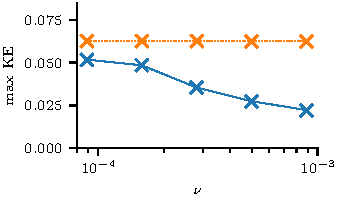
\includegraphics[width=\textwidth]{max_kinetic_changing_visc.pdf}
      \caption{Maximum kinetic energy}
    \end{subfigure}
    \caption{\textit{Anisotropic viscous heating, Ohmic heating, and maximum kinetic energy as functions of viscosity $\nu$.} Plots are shown using isotropic viscosity (blue, solid) and switching viscosity (orange, dashed) as functions of viscosity $\nu$ at the final time of $t=400$ for a fixed resistivity $\eta=5\times10^{-4.5}$, The anisotropic viscous heating has been multiplied by a factor of $10$. The maximum kinetic energy is calculated as the maximum value prior to $t=400$.}
    \label{fig:param_study_varying_viscosity}
\end{figure}

Figures~\ref{fig:param_study_varying_viscosity}(a) and~\ref{fig:param_study_varying_viscosity}(b) show the total heat generated by $t=400$ via viscous $Q_{\nu}$ and Ohmic $Q_{\eta}$ dissipation as $\nu$ is varied. It should be noted that, to allow the trend in the anisotropic viscous heating to be seen in the plot, it has been multiplied by a factor of $10$. Before discussing the apparent trends in the heating as $\nu$ is varied, it is useful to note that, just as in the typical case described previously, for the range of $\nu$ shown, isotropic viscous heating remains approximately two orders of magnitude greater than the anisotropic viscous heating, and the Ohmic heating is consistently higher when using anisotropic viscosity than when using isotropic.

Since viscous dissipation (equations~\eqref{eq:iso_viscous_heating} and~\eqref{eq:aniso_viscous_heating}) has a functional dependence on $\nu$ and Ohmic dissipation (equation~\eqref{eq:ohmic_heating}) does not, it could be naively assumed that variation in viscosity should present some trend in the viscous dissipation for both models and no trend in the Ohmic dissipation. The trends that are observed broadly adhere to this but, unexpectedly there appears some trend in the Ohmic heating when using isotropic viscosity.

When employing the switching model, the Ohmic heating appears to be independent of $\nu$, whereas when employing the isotropic model, there appears a small trend of decreased Ohmic heating with increased $\nu$. These trends can be explained by considering the effect of viscosity on compressive flows and current densities. During the kink instability, Ohmic heating, being proportional to the square of the local current density, is increased when an already sheared magnetic field is compressed by flows perpendicular to the field, increasing the local current density. Thus, as the speeds of perpendicular flows increase, so does the Ohmic heating. These perpendicular flows are effectively only damped by isotropic viscosity. Since the maximum kinetic energy (Figure~\ref{fig:param_study_varying_viscosity}(c)) decreases with $\nu$ in \emph{only} the isotropic case, and remains constant in the switching case, it is appropriate that the Ohmic heating decreases with $\nu$ in the isotropic case and is negligibly dependent on $\nu$ in the switching case.

If varying $\nu$ does not change the dynamics in the switching case, the functional dependence of $Q_{\nu}$ on $\nu$ (see equation~\eqref{eq:aniso_viscous_heating}) suggests an increase in anisotropic viscous heating with $\nu$ should be observed. Figure~\ref{fig:param_study_varying_viscosity}(a) reveals precisely this.

The relationship between the isotropic viscous heating at $\nu$ appears non-trivial. Given the decrease in maximum kinetic energy (Figure~\ref{fig:param_study_varying_viscosity}(a)) with $\nu$, it is expected the isotropic viscous heating should also decrease. However, this is not what is observed. Although there appears to be a slight decreasing trend in the isotropic viscous heating when $\nu$ is increased past $10^{-4}$, the left-most point is clearly an outlier. This suggests the secondary instability is having a significant and non-trivial effect on the heating. Indeed this is also suggested by the subtle change of gradient in the maximum kinetic energy on the left-hand side of the Figure~\ref{fig:param_study_varying_viscosity}(c). Due to this particular parameter study producing only five data points, these trends cannot be discussed with much confidence. A more detailed parameter study should be performed, investigating more values of $\nu$ within and beyond the range studied here.

\subsubsection{Dependence of linear growth rate on viscosity}
\label{sec:linear_growth_rate_varying_visc}

\begin{figure}[t]
    \centering
    \begin{subfigure}[t]{0.5\textwidth}
      \includegraphics[width=\textwidth]{growth_rate_varying_viscosity.pdf}
      \caption{Growth rate}
    \end{subfigure}%
    ~
    \begin{subfigure}[t]{0.5\textwidth}
      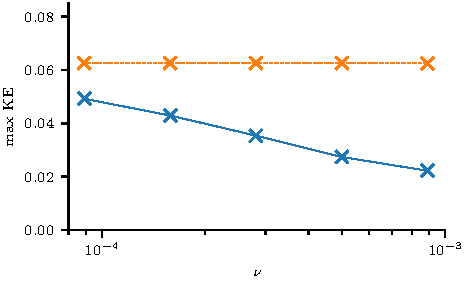
\includegraphics[width=\textwidth]{max_early_time_kinetic_changing_visc.pdf}
      \caption{Maximum early-time kinetic energy}
    \end{subfigure}
    \caption{\textit{Linear growth rate and maximum (in time) kinetic energy as
        functions of viscosity $\nu$ for a fixed
          resistivity of $\eta=5\times10^{-4.5}$.} Plots are shown using isotropic viscosity (blue, solid) and switching viscosity (orange, dashed) as functions of viscosity $\nu$. The maximum kinetic energies are calculated as the maximum values in time prior to $t=125$. This is to capture the behaviour of only the initial nonlinear evolution of the instability, neglecting any further instabilities like the secondary instability found in Section~\ref{sec:results}. Note, the maxima do not necessarily occur at the same time and this particular parameter study has been performed fixing $\nu$ at a slightly different value to the previous parameter studies.}
    \label{fig:growth_rate_varying_viscosity}
\end{figure}

For each value of $\eta$ the linear growth rate $\sigma$ of the onset of the kink instability is estimated by plotting the logarithm of the kinetic energy against time and measuring the gradient during the period of linear growth (as is done in Figure~\ref{fig:log_kinetic_energy_over_time}). Figure~\ref{fig:growth_rate_varying_viscosity}(a) plots these growth rates against $\eta$, and Figure~\ref{fig:growth_rate_varying_viscosity}(b) shows the maximum kinetic energy calculated as the maximum prior to $t=125$. For every $\eta$, this time is between the peaks of the kinetic energy corresponding to the first and secondary instabilities. Taking the maximum before this time allows us to capture only the behaviour of the initial instability, since this is the instability of interest in this section.

It can be seen from the relationship between the growth rate and $\nu$ for both viscosity models that isotropic viscosity appears to begin to suppress the kink instability, for larger $\nu$, while the switching viscosity does not (Figure~\ref{fig:growth_rate_varying_viscosity}(a)). This is also apparent from the relationship between the maximum kinetic energy and $\nu$ for both models (Figure~\ref{fig:growth_rate_varying_viscosity}(b)). This difference between the viscosity models results from the anisotropic viscosity being so weak that the dynamics of the initial onset of the kink instability are not significantly affected by a significant increase in $\nu$.

\subsection{Varying resistivity}

\subsubsection{Dependence of heating on resistivity}

\begin{figure}[t]
    \centering
    \begin{subfigure}[t]{0.5\textwidth}
      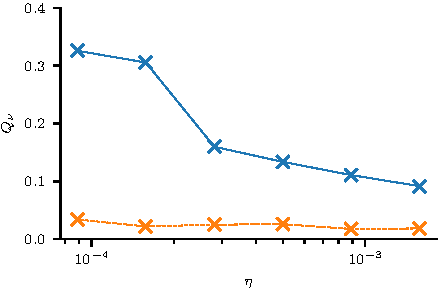
\includegraphics[width=\textwidth]{visc_heating_varying_resistivity.pdf}
      \caption{Viscous heating}
    \end{subfigure}%
    ~
    \begin{subfigure}[t]{0.5\textwidth}
      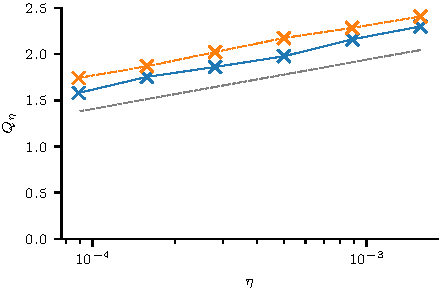
\includegraphics[width=\textwidth]{ohmic_heating_varying_resistivity.pdf}
      \caption{Ohmic heating}
    \end{subfigure}
    \caption{\textit{Anisotropic viscous, and Ohmic heating as functions of resistivity $\eta$ for a fixed value of viscosity $\nu=5\times10^{-4.5}$.} Plots are shown using isotropic viscosity (blue, solid) and switching viscosity (orange, dashed) as functions of resistivity $\eta$ at the final time of $t=400$. The anisotropic viscous heating has been multiplied by a factor of $10$. Overlaid on Figure (b) is the scaling $\log_{10}(\eta^{1/2})$.}
    \label{fig:param_study_varying_resistivity}
\end{figure}

Figure~\ref{fig:param_study_varying_resistivity}(a) and~\ref{fig:param_study_varying_resistivity}(b) show the total heating generated by $t=400$ via viscous $Q_{\nu}$ and Ohmic $Q_{\eta}$ dissipation as the strength of resistivity $\eta$ is varied. Just as in Section~\ref{sec:visc_param_study}, the anisotropic viscous heating is multiplied by $10$. Again, it is useful to note that, across the entire range of $\eta$ studied here, the isotropic viscous heating remains approximately two orders of magnitude greater than the anisotropic viscous heating and the Ohmic heating produced when using switching viscosity is consistently higher than that produced when using isotropic viscosity. This aligns with the results when varying viscosity, as discussed above.

As in the parameter study varying $\nu$, a non-trivial relationship appears between the viscous heating for both models and $\eta$ (Figure~\ref{fig:param_study_varying_resistivity}(a)). The isotropic viscous heating reveals an decreasing trend over all values of $\eta$ studies here, however there is a clear jump in heating between approximately $10^{-3.9}$ and $10^{-3.7}$. Given that these are the values of $\eta$ where there is strong influence of the secondary instability on the kinetic energy output (see Section~\ref{sec:secondary_instability}), these results suggest it is the kinetic energy produced by the secondary instability that is being damped at low values of $\eta$.

Just as in the parameter study varying $\nu$, the anisotropic viscosity shows very little variability with $\eta$ (Figure~\ref{fig:param_study_varying_resistivity}(a)), even with the heating multiplied by a factor of $10$ for plotting. Despite the dynamics significantly changing with $\eta$, the effect of the anisotropic viscosity is so small that very little change in the heating is observed.

Ohmic heating is observed to increase with increasing $\eta$ (Figure~\ref{fig:param_study_varying_resistivity}(b)). This is to be expected given the functional dependence of $Q_{\eta}$ on $\eta$, however the actual scaling is not linear in $\eta$, as might be predicted from equation~\eqref{eq:ohmic_heating}. Rather, $Q_{\nu}$ varies linearly with $\log_{10}(\eta^{1/2})$ for the range of $\eta$ studied here. Without a more comprehensive parameter study covering more values of $\eta$, it is difficult to reason why the scaling takes this form. However, what is certain is that the use of anisotropic viscosity is consistently enhancing Ohmic heating across the range of $\eta$ studied here. This is due to the kink instability producing more kinetic energy in the switching case, which better compresses the magnetic field, creating stronger current sheets and thus enhancing Ohmic heating.

\subsubsection{Dependence of linear growth rate on resistivity}

\begin{figure}[t]
    \centering
    \begin{subfigure}[t]{0.5\textwidth}
      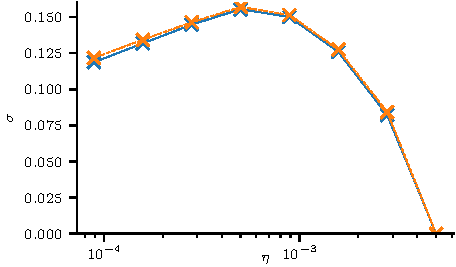
\includegraphics[width=\textwidth]{growth_rate_varying_resistivity.pdf}
      \caption{Growth rate}
    \end{subfigure}%
    ~
    \begin{subfigure}[t]{0.5\textwidth}
      \includegraphics[width=\textwidth]{max_kinetic_changing_resist.pdf}
      \caption{Maximum early-time kinetic energy}
    \end{subfigure}
    \caption{\textit{Linear growth rate and maximum (in time) kinetic energy as
        functions of resistivity $\eta$ for a fixed
          viscosity of $\nu=10^{-4}$.} \textbf{(a)} Growth rate and \textbf{(b)} maximum kinetic energy, generated by isotropic viscosity (blue, solid) and switching viscosity (orange, dashed) as functions of resistivity $\eta$. The maximum kinetic energies are calculated as the maximum values in time prior to $t=125$. This is to capture the behaviour of only the initial nonlinear evolution of the instability, neglecting any further instabilities like the secondary instability found in Section~\ref{sec:results}. Note, the maxima do not necessarily occur at the same time and this particular parameter study has been performed fixing $\nu$ at a slightly different value to the previous parameter studies.}
    \label{fig:growth_rate_varying_resistivity}
\end{figure}

As is done in Section~\ref{sec:linear_growth_rate_varying_visc}, the linear growth rates are measured for each value of $\eta$. These and the maximum early time ($t<125$) kinetic energy are shown in Figure~\ref{fig:growth_rate_varying_resistivity}. The plots show that the use of the switching model seems to consistently amplify the growth of the kink instability, shown both in the growth rate and in the kinetic energy. Beyond this, the two models of viscosity show similar trends with $\eta$.

Both plots in Figure \ref{fig:growth_rate_varying_resistivity} show that the kink instability is strongly inhibited for values of $\eta$ greater than approximately $10^{-2.5}$. This can be explained by the initial diffusion of the magnetic field being so fast-acting for large values of $\eta$ that the instability is totally suppressed. The increased suppression of the instability with strength of Ohmic diffusion can be seen in both plots as $\eta$ increases past $10^{-3}$.

\section{Discussion}

\todo{split text from summary into discussion and conclusion}

\section{Conclusion}

\section{Summary and discussion}
\label{sec:conclusions}

This chapter details the linear and nonlinear development of the MHD kink
instability with two different viscosity models. The first is
isotropic (Newtonian) viscosity, which is the most commonly used
viscosity model in coronal loop studies. The second is anisotropic viscosity, representing the strong-field limit of Bragkinskii viscosity with a preferred direction parallel to the magnetic field. The implementation of anisotropic viscosity is via the switching model~\cite{mactaggartBraginskiiMagnetohydrodynamicsArbitrary2017} which is suitable for coronal applications.

By considering particular (low) values of the viscosity and resistivity, it is found that the effect of the different viscosity models on the linear onset of the kink instability is marginal. The significant differences appear in the nonlinear phase. Two main phases of evolution can be identified which highlight the differences between the effects of the two viscosity models. The anisotropic (switching) case produces more kinetic energy at the onset of the nonlinear phase of the instability---the first phase. It also produces flows and current sheets with smaller length scales compared to the isotropic case and this allows the magnetic field to relax faster due to more efficient reconnection. 

In the second phase, the isotropic case exhibits a secondary instability, which is not found in the anisotropic case. This new instability leads to enhanced reconnection and faster magnetic relaxation, compared to the anisotropic case.  The simulations are run for $600$ Alfv\'en times (a long time period for coronal applications) and the behaviour of the second phase continues for all of this time.

A series of parameter studies was also run, where the strengths of viscosity and resistivity were varied. The qualitative results of the two phases of the detailed investigation hold true over a range of viscosities and resistivities, including the existence of the secondary instability. Notably, over all parameters studied, viscous heating is consistently overestimated by the isotropic model, and Ohmic heating is consistently enhanced by use of the switching model.

Although there can be much variability in the nonlinear behaviour of the kink instability, these results reveal an important general finding. At the beginning of the nonlinear phase, anisotropic (parallel) viscosity allows for the development of smaller length scales (both flows and current sheets), compared to isotropic viscosity, leading to more efficient reconnection and faster magnetic relaxation, at least initially. As has been described in detail, isotropic viscosity can produce other effects later. However, for coronal applications, it is the initial nonlinear phase of the instability that is likely to be of most interest since, in reality, a coronal loop will interact with others on a longer time scale, thus affecting the nonlinear evolution. Since anisotropic viscosity is a more realistic model for viscosity in the corona, these results will be useful in the interpretation of observations of coronal loops that are kink unstable.

% and the other chapters
\appendix
\chapter{Software and reproduction of results}

This thesis has involved the development of a number of tools used to analyse the outputs from Lare3d, mostly written in Python. For the purpose of proper reproducibility, this appendix details the theory behind the field line integrator, the precise software versions and parameters used to run the simulations and analyses, and the locations of all relevant code and data. Due to the size of the output files from Lare3d (the total amount of data generated in the entire thesis is approximately 10 TB) only the code and relevant parameters are published. These should provide enough information to reproduce the simulation results, however if a required piece is missing, I encourage the reader to contact me.

\section{Reproduction of results}

With the exception of a field line integrator used in chapter~\ref{chp:kink_instability}, all analysis code is packaged alongside the latex files used to generate this thesis and can be found in the Github repository at \url{https://github.com/jamiejquinn/thesis} and is also stored in Zenodo\todo{cite thesis}. The theory behind each piece of analysis is described in the relevant chapters and instructions for rerunning any analysis can be found in the README of the thesis repository. The field line integrator used in chapter~\ref{chp:kink_instability} can be found at~\cite{jamie_j_quinn_2019_3560249} and is distinct from the alternative field line integrator used in other chapters which is described below and can be found alongside the other analysis tools in the thesis repository.

The code which implements only the anisotropic viscosity module can be found at~\cite{keith_bennett_2020_4155546} and should be simple to merge into another version of Lare3d for future research. To facilitate reproduction of the simulation data presented in this thesis, the code used in each chapter is individually packaged in different branches of the repository found at \url{https://github.com/jamiejquinn/Lare3d} and are also stored in Zenodo for chapter~\ref{chp:switching_model} at~\cite{keith_bennett_2020_4155661}, chapter at~\ref{chp:kink_instability} at~\cite{keith_bennett_2020_4155670}, chapter~\ref{chp:kink_instability_straight} at~\cite{keith_bennett_2020_4155625}, and chapter~\ref{chp:null_point_khi} at~\cite{keith_bennett_2020_4155646}. These versions of Lare3d include initial conditions, boundary conditions and basic running parameters. The specific parameters used in each individual simulation can be found in the methods sections of the corresponding chapters. The parameters were inputted to the simulations using the tools found in the \verb|run_scripts| folder of the thesis repository. These can be used to quickly generate multiple simulations suitable for a parameter study.

All simulations were performed on a single, multi-core machine with $40$ cores and $192$ GB of RAM, although this amount of RAM is much higher than was required; a conservative estimate of the memory used in the largest simulations is around $64$ GB. Most simulations completed in under $2$ days, although the longest running simulations (the highest-resolution cases in chapter~\ref{chp:null_point_khi}) completed in around $2$ weeks. 

\section{Field line integrator}

As detailed in section~\ref{sec:kink_methods_analysis}, the reconnection rate local to a single field line is given by the electric field parallel to the magnetic field, integrated along the field line. The global reconnection rate for a given region of magnetic diffusion is the maximum value of the local reconnection rate over all field lines threading the region. In chapter~\ref{chp:kink_instability} this was calculated using the visualisation tool Mayavi (more details are found in section~\ref{sec:kink_methods_analysis}) while in all other chapters, a field line integrator was developed specifically for the calculation of reconnection rate and is detailed here.

Magnetic field lines lie tangential to the local magnetic field at every point $\vec{x}(s)$ along the line,
\begin{equation}
  \label{eq:field_line_equation}
  \frac{d\vec{x}(s)}{ds} = \vec{b}(\vec{x}(s)),
\end{equation}
where $s$ is a variable which tracks along a single field line and $\vec{b}$ is the unit vector in the direction of $\vec{B}$. This equation is discretised using a second-order Runge-Kutta scheme to iteratively calculate the discrete positions $\vec{x}_i$ along a field line passing through some seed position $\vec{x}_0$,
\begin{align}
  \label{eq:field_line_calculation}
  \vec{x}_{i+1} &= \vec{x}_i + h\vec{b}(\vec{x}'_i),\\
  \vec{x}'_i &= \vec{x}_i + \tfrac{h}{2}\vec{b}(\vec{x}_i)
\end{align}
where $h$ is a small step size. Since $\vec{b}$ is discretised, the value at an arbitrary location $\vec{x}_i$ is calculated using a linear approximation. The integration of a scalar variable $y$ is carried out along a field line given by a sequence of $N$ locations $\vec{x}_i$ using the midpoint rule,
\begin{equation}
  \label{eq:midpoint_rule}
  Y = \sum_{i=1}^{i=N} \frac{(y(\vec{x}_{i-1}) + y(\vec{x}_{i}))}{2},
\end{equation}
where $Y$ is the result of the integration. In practice, $N$ is not specified and the discretised field line contains the required number of points to thread from its seed location to the boundary of the domain.

While the linear interpolation, second-order Runge-Kutta and midpoint rule are all low order methods, testing higher-order methods showed little change in results but dramatically increased the runtime of the analysis. The lower-order methods used offer an acceptable compromise between speed and accuracy. The above algorithm is implemented in Python and can be found in \verb|code/shared/field_line_integrator.py| with examples of use in \verb|code/null_point_khi/field_line_integrator.Rmd|. The integration of multiple field lines is an embarrassingly parallel problem and is parallelised in a straight-forward manner using a pool of threads supplied by the \verb|Pool| feature of the Python library \verb|multiprocessing|. Although the integrator is solely used to integrate the parallel electric field along magnetic field lines in this thesis, the tool can be easily applied to arbitrary vector and scalar fields.


\backmatter  % Turn off chapter numbering
% I assume that the bibliography is assembled by hand.
% Change the file if you use bibtex or something like that.
\printbibliography

\end{document}
